\chapter{Applicazioni}
\label{cap:applicazioni}

Le applicazioni di questo lavoro di tesi sono mirate alla valutazione
dell'energia di correlazione calcolata con la teoria NEV-PT su
varie classi di sistemi: composti carbonilici, 
molecole $\pi$ coniugate cicliche e molecole $\pi$ coniugate lineari. Le
valutazioni sono state effettuate sia nello stato fondamentale che in alcuni
stati eccitati di singoletto. Le classi di composti in questione sono state
scelte per il ruolo centrale che svolgono nell'ambito organico, inorganico,
biologico e farmacologico.  

\section{Sistemi carbonilici semplici}

Lo studio dei sistemi carbonilici si \`e concentrato sulla valutazione
dell'energia di eccitazione $n \rightarrow \pistar$ su formaldeide,
acetaldeide ed acetone, per le transizioni singoletto-singoletto
verticale ed adiabatica. L'analisi \`e stata effettuata con basi di diversa
dimensionalit\`a, su uno spazio CAS con 6 elettroni attivi in 5 orbitali attivi,
ad eccezione dell'acetaldeide,
per la quale \`e stato utilizzato uno spazio CAS di dimensionalit\`a maggiore
al fine di ottenere risultati comparabili al dato sperimentale, dal momento che
la sua intrinseca asimmetria comportava problemi nell'utilizzo di uno spazio
CAS ridotto.

\subsection{Formaldeide}

\subsubsection{Ottimizzazione geometrica e simmetria}

Abbiamo considerato la formaldeide in quanto essa risulta il composto
organico pi\`u semplice
per la trattazione \textit{ab initio} del gruppo carbonilico. 

Come punto di partenza per l'approccio computazionale si \`e fatto uso di
una geometria sperimentale, successivamente ottimizzata mediante il programma
\texttt{dalton}. La tabella \ref{tab:geom_formaldeide} mostra i parametri geometrici
caratteristici della formaldeide nello stato fondamentale, ottimizzati con
differenti metodi nella base 6-311G*

\begin{center}
\begin{threeparttable}
\caption{\small Formaldeide - geometrie di equilibrio}
\label{tab:geom_formaldeide}
\small
\begin{tabular}{|c|ccc|}
\hline
					& HF			& CAS			 	&  Exp.\tnote{1} \\
\hline
$r$(C-O)			&  1.1782		& 1.2161			&  1.2078 \\
$r$(C-H)			&  1.0936	 	& 1.0885 			&  1.1161 \\
$\angle$(H-C-H)		&  115.94 	 	& 117.20			&  116.50 \\
$\angle$(H-C-O)		&  122.03 	 	& 121.40			&  121.75 \\
Energia				&  1.895765 	& 1.968732			&         \\
\hline
\end{tabular}
\begin{tablenotes}
 \item[1] \small Cfr. \cite{jpsj-18-1963-1174} e \cite{jpc-97-17-1993-4293}
 \item[] \small Valori in Angstroms. Angoli in gradi. Energia come \mbox{-(112 + valore)} Hartree.

\end{tablenotes}
\end{threeparttable}
\end{center}

Possiamo notare come i risultati ottenuti a livello CASSCF siano in
migliore accordo con i valori sperimentali rispetto ai risultati ottenuti a
livello HF.
Il sistema appartiene al gruppo di simmetria C$_{2v}$, la cui tavola dei
caratteri \`e qui rappresentata

\begin{center}
\begin{tabular}{c|cccc|c|c}
  $C_{2v}$  & E &  $C_2$ & $\sigma_{xz}$ & $\sigma_{yz}$ &  &  \\
\hline
    $A_1$  &   1 &   1 &   1 &   1 & z & $x^2$, $y^2$, $z^2$ \\
    $B_1$  &   1 &  -1 &   1 &  -1 & x, $R_y$ & xz \\
    $B_2$  &   1 &  -1 &  -1 &   1 & y, $R_x$ & yz \\
    $A_2$  &   1 &   1 &  -1 &  -1 & $R_z$ & xy \\
\end{tabular}
\end{center}

La molecola \`e disposta sul piano $yz$, con l'asse C$_2$ colineare all'asse $z$.

Il calcolo CAS fa riferimento ad un sistema con 6 elettroni attivi in uno
spazio di 5 orbitali. La figura \ref{fig:formaldeide_orbitali} mostra
le forme degli orbitali e le rispettive simmetrie.
\begin{figure}[htb]
\begin{center}
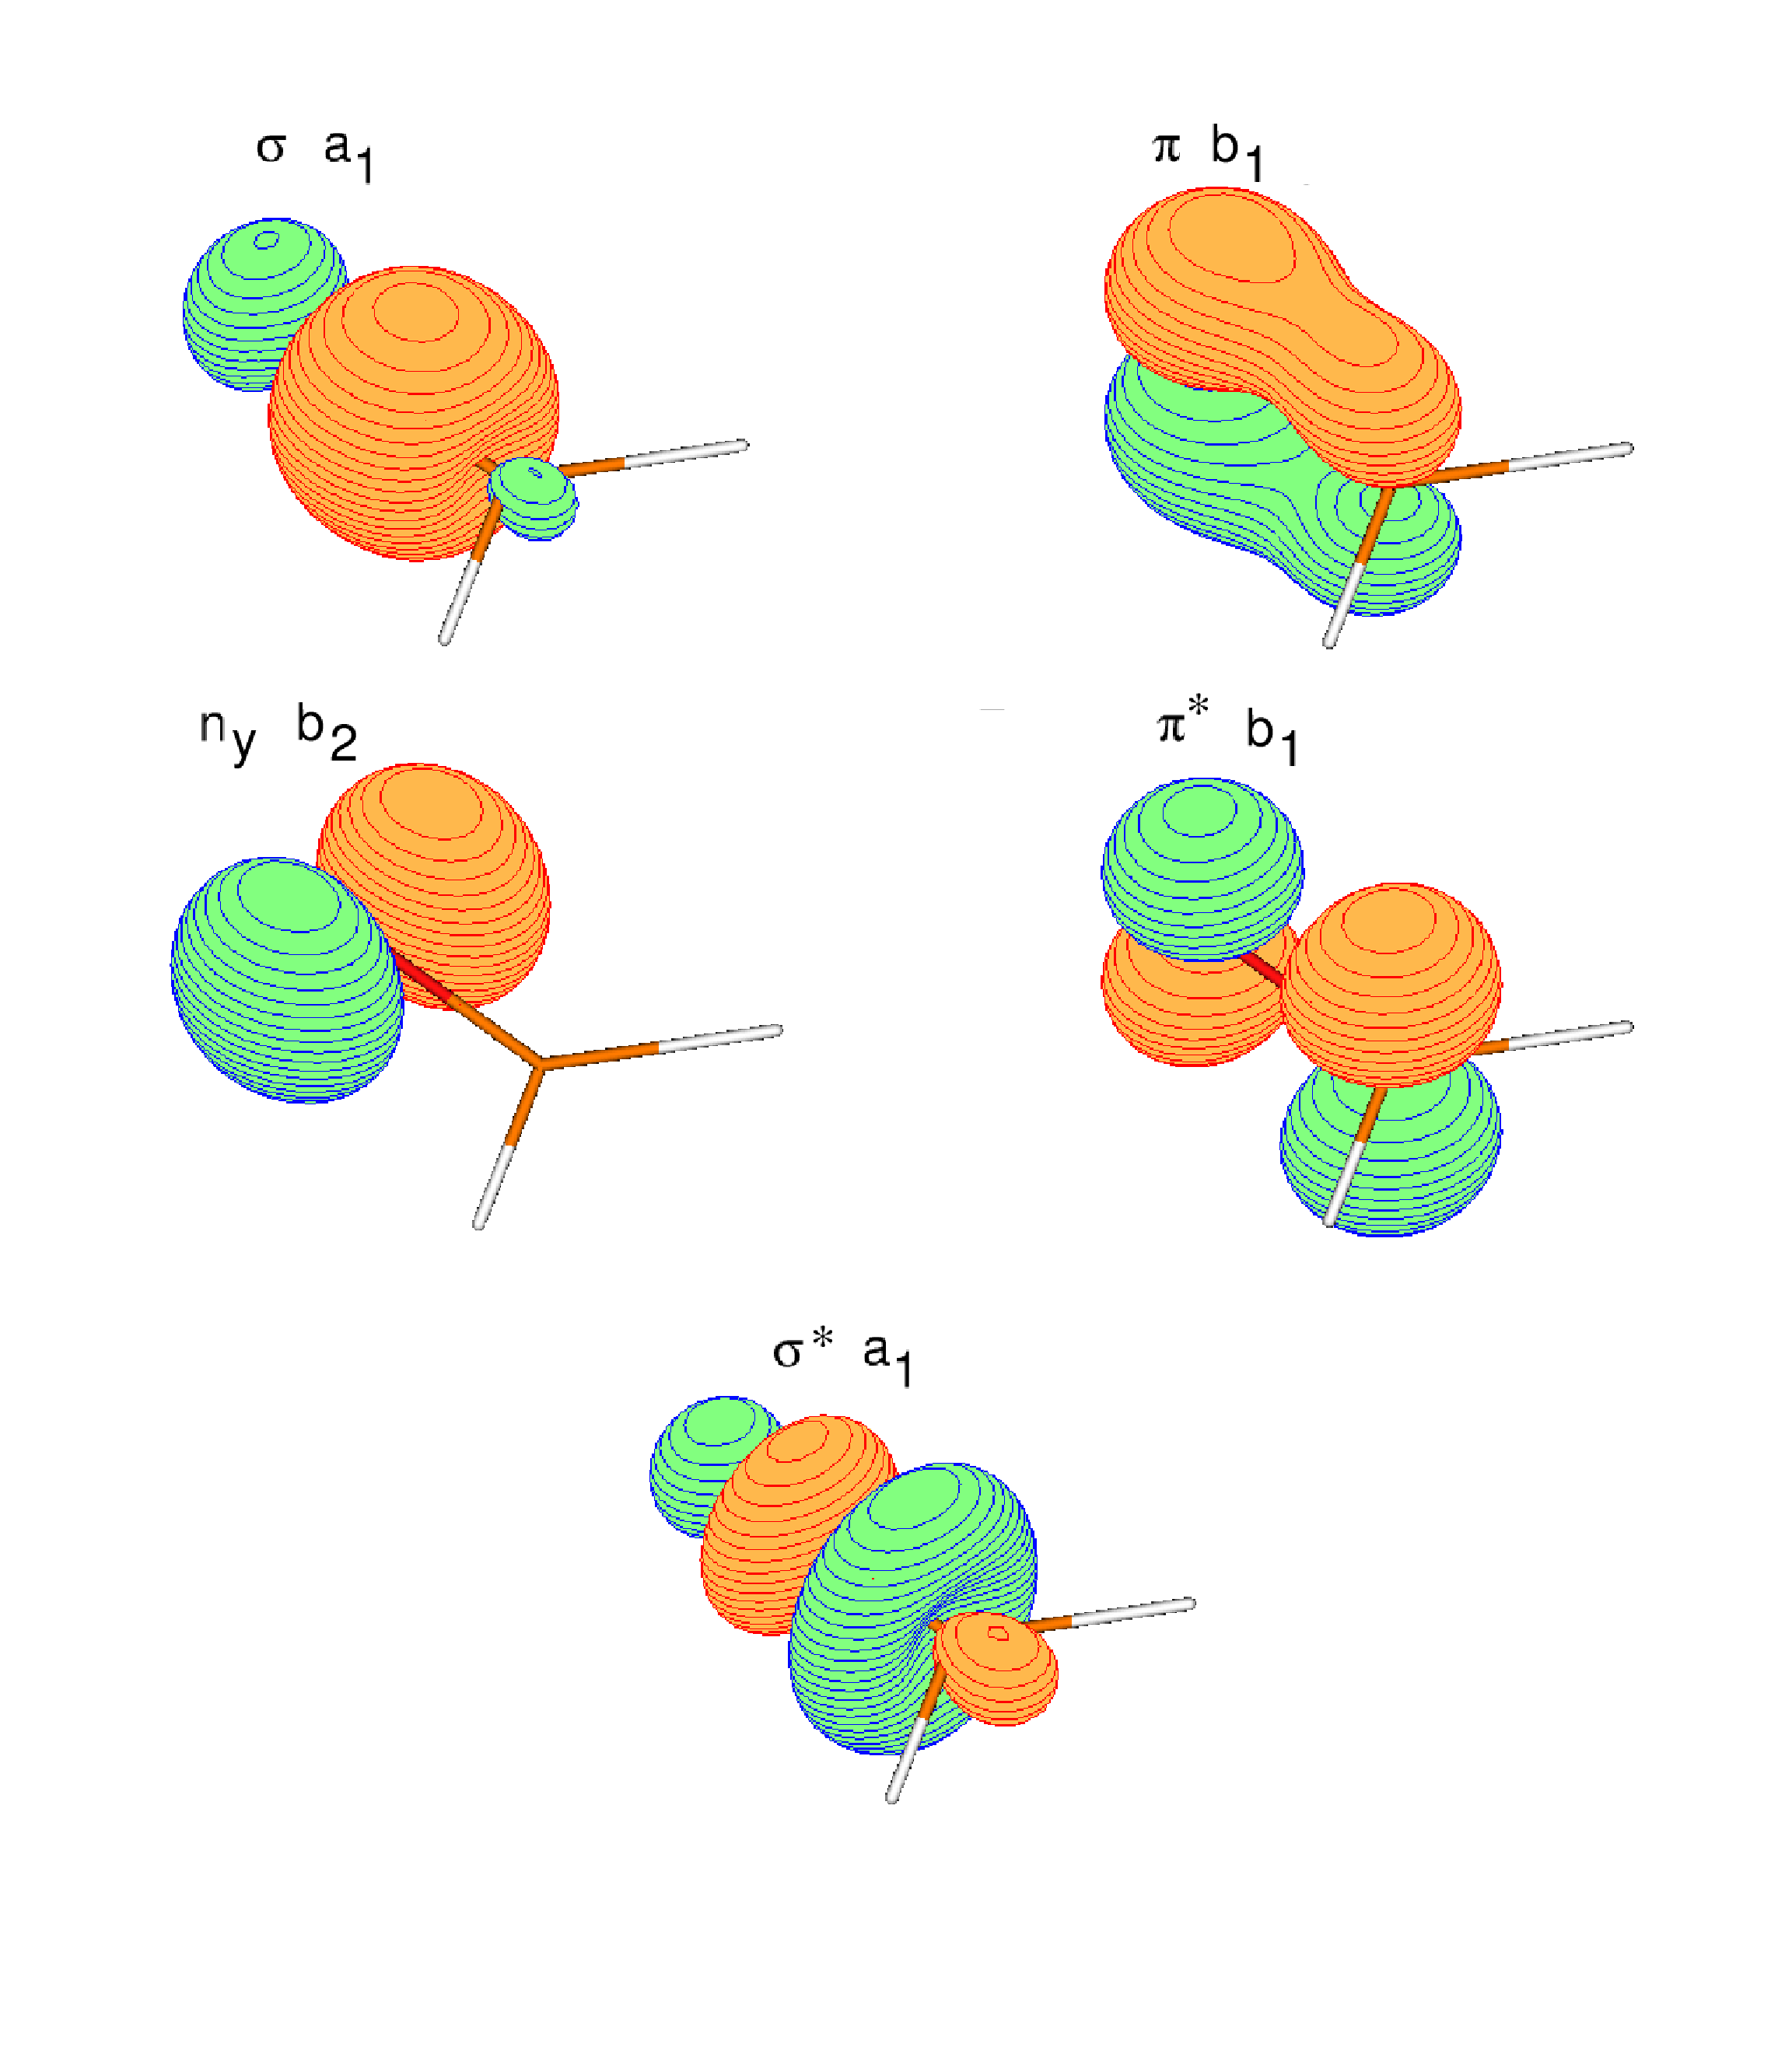
\includegraphics[width=8cm,keepaspectratio]{immagini/formaldeide/orbitali.eps}
\end{center}
\caption{Spazio CAS per la formaldeide}
\label{fig:formaldeide_orbitali}
\end{figure}

Nella trattazione HF gli orbitali doppiamente occupati sono
\begin{itemize}
\item 5 di simmetria A$_1$
\item 1 di simmetria B$_1$
\item 2 di simmetria B$_2$
\end{itemize}
Lo spazio CAS \`e stato costruito utilizzando, per lo spazio di core
(doppiamente occupato) 4 orbitali A$_1$ e 1 orbitale B$_2$,
mentre lo spazio attivo \`e stato definito da 2 orbitali A$_1$
(l'orbitale legante $\sigma$ e l'antilegante $\sigma^{*}$), 2 orbitali B$_1$
(un legante $\pi$ e l'antilegante $\pistar$) e 1 orbitale B$_2$ (non legante 
$n_y$), con 6 elettroni attivi e 10 elettroni di core.
Con questa scelta, sono necessarie 18 configurazioni per descrivere la molecola
nello stato fondamentale (simmetria A$_1$). 

Nel caso della transizione elettronica di interesse, si avr\`a la promozione
di un elettrone dall'orbitale $n_y$, di simmetria B$_2$, all'orbitale $\pistar$,
di simmetria B$_1$. La tabella dei prodotti diretti delle rappresentazioni
per il gruppo C$_{2v}$ 
\begin{center}
\begin{tabular}{|c|cccc|}
\hline
 C$_{2v}$ & A$_1$ & B$_1$ & B$_2$ & A$_2$ \\
\hline                                
    A$_1$ & A$_1$ &       &       &        \\
    B$_1$ & B$_1$ & A$_1$ &       &        \\
    B$_2$ & B$_2$ & A$_2$ & A$_1$ &        \\
    A$_2$ & A$_2$ & B$_2$ & B$_1$ & A$_1$  \\
\hline
\end{tabular}
\end{center}
indica per lo stato elettronico finale la simmetria B$_2 \otimes $B$_1 = $A$_2 $.

Il calcolo ha fornito, per lo spazio attivo del ground state, i seguenti numeri
di occupazione
\begin{verbatim}
 Simmetria A1 : 1.978929123   0.021519393
 Simmetria B1 : 1.929961079   0.070506119
 Simmetria B2 : 1.999084286
\end{verbatim}

L'energia CASSCF finale \`e -113.968732 Hartree, che si assume come energia
del ground state per il calcolo della transizione sulla base 6-311G*
a livello CASSCF.

%Limitatamente alla molecola di formaldeide sono state inoltre calcolate le
%energie di eccitazione per le transizioni $n_z \rightarrow \pistar$ e $\pi \rightarrow
%\pistar$, che comportano uno stato elettronico finale di simmetria $A_1 \otimes B_1 = B_1$
%e $B_1 \otimes B_1 = A_1$ rispettivamente. Di conseguenza, nel caso della
%transizione $\pi \rightarrow \pistar$, non avviene cambiamento di simmetria, dal momento
%che il ground state \`e anch'esso di simmetria $A_1$. L'energia dello stato eccitato
%sar\`a quindi la seconda radice della diagonalizzazione nella simmetria del ground state.

%In tabella \ref{tab:formaldeide_vertical} riportiamo i valori ottenuti per le varie transizioni,
%affiancate al dato sperimentale
%\begin{center}
%\begin{threeparttable}
%\caption{Formaldeide - energie di transizione verticale CAS/6-311G*}
%\label{tab:formaldeide_vertical}
%\small
%\begin{tabular}{|ccccc|}
%\hline
%							& Simm.		& Energia\tnote{1}	& Eccitato - GS\tnote{2} & Sperim.\tnote{2} \\
%\hline
%$GS$ 						& A1		& 1.96873 			& 0		& 0   \\
%$n_y \rightarrow \pistar$ 	& A2		& 1.80577 			& 4.43  & 4.07 \\
%$n_z \rightarrow \pistar$ 	& B1		& 1.59497			& 10.17 & 9.97 \tnote{3} \\
%$\pi \rightarrow \pistar$   & A1        & 1.55132           & 11.36 & 9.19 \tnote{3} \\
%\hline
%\end{tabular}
%\begin{tablenotes}
%\tiny
% \item[1] Energia come - (112 + valore) Hartree.
% \item[2] Valore in eV
% \item[3] Valore sperimentale non disponibile. Dati da CIS-MP2 su 6-311(2+,2+)G** (Cfr. \cite{jpc-97-17-1993-4293})
%\end{tablenotes}
%\end{threeparttable}
%\end{center}

Il calcolo effettuato sullo stato eccitato di simmetria A$_2$, mantenendo la
geometria ottimizzata per lo stato fondamentale (transizione verticale) ha fornito
invece un'energia di -113.80577 Hartree, comportando di conseguenza un'energia di
transizione elettronica pari a 4.43 eV, che confrontato al valore sperimentale
4.07 eV (Cfr. \cite{jpc-99-20-1995-8050}) evidenzia un errore di circa 0.4 eV. 
%Le altre transizioni non sono esattamente
%definite, e non vi sono ancora riferimenti bibliografici certi sull'assegnazione energetica
%della transizione $\pi \rightarrow \pistar$, che dovrebbe giacere tra i 9 e gli 11 eV. (Cfr.
%\cite{jpc-99-20-1995-8050}). Per questa ragione, tali calcoli non verranno affrontati su molecole
%pi\`u complesse, ma limiteremo il nostro studio alla sola transizione verticale e adiabatica
%$n_y \rightarrow \pistar$.

I numeri di occupazione confermano la transizione $n_y \rightarrow \pistar$
\begin{verbatim}
 Simmetria A1 : 1.984641659   0.015707156
 Simmetria B1 : 1.996255549   1.003395636
 Simmetria B2 : 1.000000000
\end{verbatim}

\`E stata successivamente condotta un'ottimizzazione di geometria per lo
stato eccitato, valutando di conseguenza la transizione adiabatica. In tali
condizioni, la simmetria del sistema cala da C$_{2v}$ a C$_s$, venendo a
mancare un piano di riflessione in seguito alla piramidalizzazione della
molecola.

\begin{center}
\begin{threeparttable}
\caption{\small Formaldeide - geometrie di transizione adiabatica}
\label{tab:formaldeide_geometrie_adiab}
\begin{tabular}{|c|cc|}
\hline
					& GS		& $n_y \rightarrow \pistar$ \\ %& $n_z \rightarrow \pistar$	\\
\hline
$r$(C-O)		 	& 1.2161	&  1.3817 				\\ %& 1.541100 					 \\
$r$(C-H)			& 1.0885	&  1.0762					\\ %& 1.078499					 \\
$\angle$(H-C-H)		& 117.20	&  119.44					\\ %& 115.812					 \\
$\angle$(H-C-O)		& 121.40	&  113.03					\\ %& 110.473					 \\
Energia 			& 1.968732	&  1.834522					\\ %& 1.673067					 \\
En. Eccitazione 	& 			&  3.65						\\ %& 8.04						 \\
En. Ecc. Exp.\tnote{1} & 	&  3.50						\\ %& 8.49						 \\
\hline
\end{tabular}
\begin{tablenotes}
\small
 \item[1] Cfr. \cite{sa-34a-1978-749} e \cite{jpc-97-17-1993-4293}
 \item[] Valori in Angstroms, angoli in gradi, Energie assolute come
  \mbox{-(112 + valore)} Hartree, energie di eccitazione in eV
\end{tablenotes}
\end{threeparttable}
\end{center}

La geometria da planare muta in piramidale. \`E osservabile uno spostamento
degli atomi di idrogeno fuori dal piano molecolare ed un allungamento del
legame C-O dovuto all'occupazione di un orbitale di antilegame $\pistar$,
accompagnato da una netta diminuzione dell'angolo di legame H-C-O verso
valori caratteristici di una geometria piramidale.

A causa del calo di simmetria del sistema, gli orbitali precedentemente
riconducibili alle rappresentazioni A$_1$ e B$_1$ appartengono ora alla
rappresentazione A$^{\prime}$, mentre gli orbitali appartenenti alle 
rappresentazioni B$_2$ e A$_2$ ora saranno di simmetria A$^{\prime\prime}$.
Lo spazio attivo precedentemente definito vedr\`a di conseguenza, 
$\sigma$, $\sigma^{*}$, $\pi$ e $\pistar$ appartenere ad A$^{\prime}$,
e $n_y$ ad A$^{\prime\prime}$. Una transizione elettronica $n_y \rightarrow
\pistar$ avr\`a simmetria A$^{\prime\prime} \otimes $A$^{\prime} =
$A$^{\prime\prime}$

Lo stato eccitato ha un'energia CASSCF pari a -113.834522
Hartree, che comporta un'energia di transizione di 3.65 eV, contro un valore
sperimentale di 3.50 eV (Cfr. \cite{jpc-97-17-1993-4293} e \cite{sa-34a-1978-749})

\subsubsection{Dipendenza dalla base atomica}

Per valutare la dipendenza dalla base atomica utilizzata si sono effettuati calcoli per
le transizioni verticale e adiabatica $ n_y \rightarrow \pistar $ su differenti 
set di base, in ordine di dimensionalit\`a:
\begin{itemize}
 \item 6-31G (Cfr. \cite{mp-27-1974-209})
 \item cc-pVDZ (Cfr. \cite{jcp-90-1989-1007})
 \item ano-1 (Cfr. \cite{jcp-55-1971-4798}) con riduzione 3s2p1d per il carbonio e 2s1p per l'idrogeno
 \item 6-311G* (Cfr. \cite{jcp-72-1980-5639})
 \item cc-pVTZ (Cfr. \cite{jcp-90-1989-1007})
 \item cc-pVQZ (Cfr. \cite{jcp-90-1989-1007})
\end{itemize}
Su ogni base \`e stata effettuata una ottimizzazione di geometria della
molecola, a livello CASSCF.

La tabella \ref{tab:formaldeide_vertical_basis} riporta i risultati ottenuti
per la transizione verticale. \`E evidente come basi a dimensionalit\`a molto
elevata, come cc-pVTZ e cc-pVQZ, portino a risultati pressoch\'e identici.
\`E quindi prevedibile che una ulteriore estensione della base non fornirebbe
risultati pi\`u accurati di quelli ottenuti, e comporterebbe un notevole incremento
dei tempi di calcolo. L'errore commesso a livello CASSCF resta
considerevole, essendo di 0.34 eV.  Una possibile soluzione alternativa \`e
ricercabile nell'allargamento dello spazio CAS, che aumenterebbe in modo
deciso la complessit\`a computazionale.

Di conseguenza, per cercare di migliorare i risultati CASSCF abbiamo
condotto dei calcoli perturbativi utilizzando la teoria NEV-PT, ottenendo
ottimi risultati con tempi di calcolo pi\`u che accettabili. La
tabella \ref{tab:formaldeide_vertical_basis} mostra quanto ottenuto, sia per
l'approccio Strongly Contracted (NEV-PT/SC) che per quello Partially Contracted
(NEV-PT/PC).

\begin{center}
\begin{threeparttable}
\caption{\small Formaldeide - Energia di transizione $n_y \rightarrow \pistar$ verticale di singoletto, metodi CASSCF e CASSCF/NEV-PT}
\label{tab:formaldeide_vertical_basis}
{
\small
\begin{tabular}{|c|ccc|ccc|}
\hline
 Base	& \multicolumn{3}{c}{GS\tnote{1}}				& \multicolumn{3}{c|}{$n_y \rightarrow \pistar$ vert.\tnote{2}} \\
		& CASSCF		& NEV-PT & NEV-PT	& CASSCF		& NEV-PT & NEV-PT \\
		& 				& SC	 & PC		& 				& SC 	& PC \\
\hline
6-31G	& 1.891188		& 2.019821		& 2.021959		& 3.85			& 3.73		& 3.72		    \\
cc-pVDZ	& 1.950044		& 2.183100		& 2.185533		& 4.38			& 4.07 		& 4.10			\\
ano-1	& 1.978883		& 2.207808		& 2.210750		& 4.36			& 4.02 		& 4.01			\\
6-311G*	& 1.968732		& 2.242321		& 2.244788		& 4.43 			& 4.07		& 4.11 			\\
cc-pVTZ & 1.985284 		& 2.316323		& 2.319135		& 4.40			& 4.04 		& 4.02			\\
cc-pVQZ & 1.994326		& 2.381916		& 2.384828		& 4.41			& 4.04		& 4.02			\\
\hline
\hline
Exp.	&				& 				&				& \multicolumn{3}{c|}{4.07} \\
\hline
\end{tabular}
}
\begin{tablenotes}
\small
 \item[1] Energia come -(112 + valore) Hartree
 \item[2] Valori in eV
\end{tablenotes}
\end{threeparttable}
\end{center}

Per quanto riguarda la transizione adiabatica, si \`e tenuto conto della differenza
tra le energie di punto zero (Zero Point Energy, ZPE) dei due stati elettronici. Questa differenza deriva
dalla diversa struttura della superficie di potenziale per lo stato fondamentale ed
eccitato, che si riflette in una diversa energia dello stato vibrazionale
fondamentale per i due stati elettronici. Assumendo che l'effetto perturbativo non attui modifiche
significative sulla struttura del potenziale CASSCF, ma si limiti ad una
traslazione energetica omogenea, le energie di punto zero per i calcoli
perturbativi possono essere assunte uguali a quella CASSCF. 
Ci\`o non \`e strettamente garantito, tuttavia \`e una approssimazione necessaria,
in quanto una accurata valutazione di questo effetto necessiterebbe di un
calcolo accurato di tutta la superficie di potenziale a livello
perturbativo.
Per questa ragione, la correzione ZPE
\`e stata applicata allo stesso modo sia sul calcolo CASSCF che sul calcolo 
perturbativo.

\begin{center}
\begin{threeparttable}
\caption{\small Formaldeide - Energia di transizione $n_y \rightarrow \pistar$ adiabatica di singoletto, calcolata a livello CASSCF e NEV-PT}
\label{tab:formaldeide_basis_energy}
{
\small
\begin{tabular}{|c|cccccc|}
\hline
Base	& ZPE 			& ZPE 				& $\Delta$ZPE	& CASSCF	& NEV-PT	& NEV-PT \\
		& (GS)			& (Ecc.)			& 				& ZPE 		&   SC/ZPE 	& PC/ZPE \\
\hline
6-31G	& 0.766			& 0.685				& -0.081		&  3.13		& 3.12			  & 3.14			\\
cc-pVDZ & 0.760			& 0.692				& -0.068        &  3.56		& 3.49			  & 3.50			\\
ano-1	& 0.764			& 0.696				& -0.068		&  3.55		& 3.43			  & 3.45			\\
6-311G* & 0.765			& 0.700				& -0.066		&  3.59		& 3.52			  & 3.57			\\
cc-pVTZ & 0.759         & 0.692				& -0.067		&  3.60		& 3.55			  & 3.56			\\
cc-pVQZ & 0.760			& 0.693				& -0.067		&  3.61		& 3.58			  & 3.59			\\
\hline
\hline
Exp.	&				& 					& 				& \multicolumn{3}{c|}{3.50}						\\
\hline
\end{tabular}
}
\begin{tablenotes}
\small
 \item[ ] Valori in eV
\end{tablenotes}
\end{threeparttable}
\end{center}

In figura \ref{fig:formaldeide_gs} sono rappresentate le energie elettroniche del
ground state a livello CASSCF (linea rossa), NEV-PT/SC (linea verde) e
NEV-PT/PC (linea blu), in funzione della base atomica scelta, in ordine di
dimensionalit\`a. Come si pu\`o notare, la NEV-PT/SC fornisce
risultati di pochissimo superiori in energia alla NEV-PT/PC.

\begin{figure}[ht]
\begin{center}
\includegraphics[angle=270,width=10cm,keepaspectratio]{immagini/formaldeide/gs.eps}
\parbox[h]{10cm}{
\caption{\small Formaldeide - Energia dello stato fondamentale a livello CASSCF (linea rossa),
NEV-PT/SC (linea verde) e NEV-PT/PC (linea blu). }
\label{fig:formaldeide_gs}
}
\end{center}
\end{figure}
\clearpage

Analogamente, le figure \ref{fig:formaldeide_vert} e
\ref{fig:formaldeide_adiab} forniscono la medesima rappresentazione
relativamente agli stati eccitati calcolati alla geometria di equilibrio
dello stato fondamentale e dello stato eccitato rispettivamente. 

\begin{figure}[ht]
\begin{center}
\includegraphics[angle=270,width=7cm,keepaspectratio]{immagini/formaldeide/vert.eps}
\parbox[h]{12cm}{
\caption{\small Formaldeide - Energia dello stato eccitato (transizione verticale)
a livello CASSCF (linea rossa), NEV-PT/SC (linea verde) e NEV-PT/PC (linea blu) come
funzione della base atomica. }
\label{fig:formaldeide_vert}
}
\end{center}
\end{figure}
\begin{figure}[ht]
\begin{center}
\includegraphics[angle=270,width=7cm,keepaspectratio]{immagini/formaldeide/adiab.eps}
\parbox[h]{12cm}{
\caption{\small Formaldeide - Energia dello stato eccitato (transizione
adiabatica) a livello CASSCF (linea rossa), NEV-PT/SC (linea verde) e NEV-PT/PC (linea blu) come
funzione della base atomica. }
\label{fig:formaldeide_adiab}
}
\end{center}
\end{figure}
\clearpage

Diagrammando l'energia della transizione verticale contro la base, si ottiene
il grafico in figura \ref{fig:formaldeide_energie_vert}. La simbologia
utilizzata \`e analoga a quella della figura precedente. La linea viola denota
il valore sperimentale di $4.07$ eV.

\begin{figure}[ht]
\begin{center}
\includegraphics[angle=270,width=12cm,keepaspectratio]{immagini/formaldeide/energie_vert.eps}
\parbox[h]{12cm}{
\caption{\small Formaldeide - energia di transizione verticale su basi differenti a livello CASSCF (linea rossa), NEV-PT/SC (linea verde) e NEV-PT/PC (linea blu) come funzione della base atomica.}
\label{fig:formaldeide_energie_vert}
}
\end{center}
\end{figure}

\`E possibile vedere come la transizione verticale venga descritta con buona accuratezza
anche con basi piccole, una volta che si sia introdotta la correzione perturbativa.
\clearpage

L'energia della transizione adiabatica in figura
\ref{fig:formaldeide_energie_adiab} mostra invece l'andamento di tale
parametro contro il valore sperimentale di $3.50$ eV.

\begin{figure}[ht]
\begin{center}
\includegraphics[angle=270,width=12cm,keepaspectratio]{immagini/formaldeide/energie_adiab.eps}
\parbox[h]{12cm}{
\caption{\small Formaldeide - energia di transizione adiabatica su basi differenti a livello CASSCF (linea rossa), NEV-PT/SC (linea verde) e NEV-PT/PC (linea blu) come funzione della base atomica.}
\label{fig:formaldeide_energie_adiab}
}
\end{center}
\end{figure}

\clearpage

%%%%%%%%%%%%%%%%%%%%%%%%%%%%%%%%%%%%%%%%%%%%%%%

\subsection{Acetone}

Analoga trattazione \`e stata effettuata nel caso della molecola di acetone.
La geometria iniziale, fornita attraverso z-matrix, possiede configurazione C$_{2v}$,
con gli atomi di idrogeno metilici sul piano, non affacciati.

\begin{figure}[ht]
\begin{center}
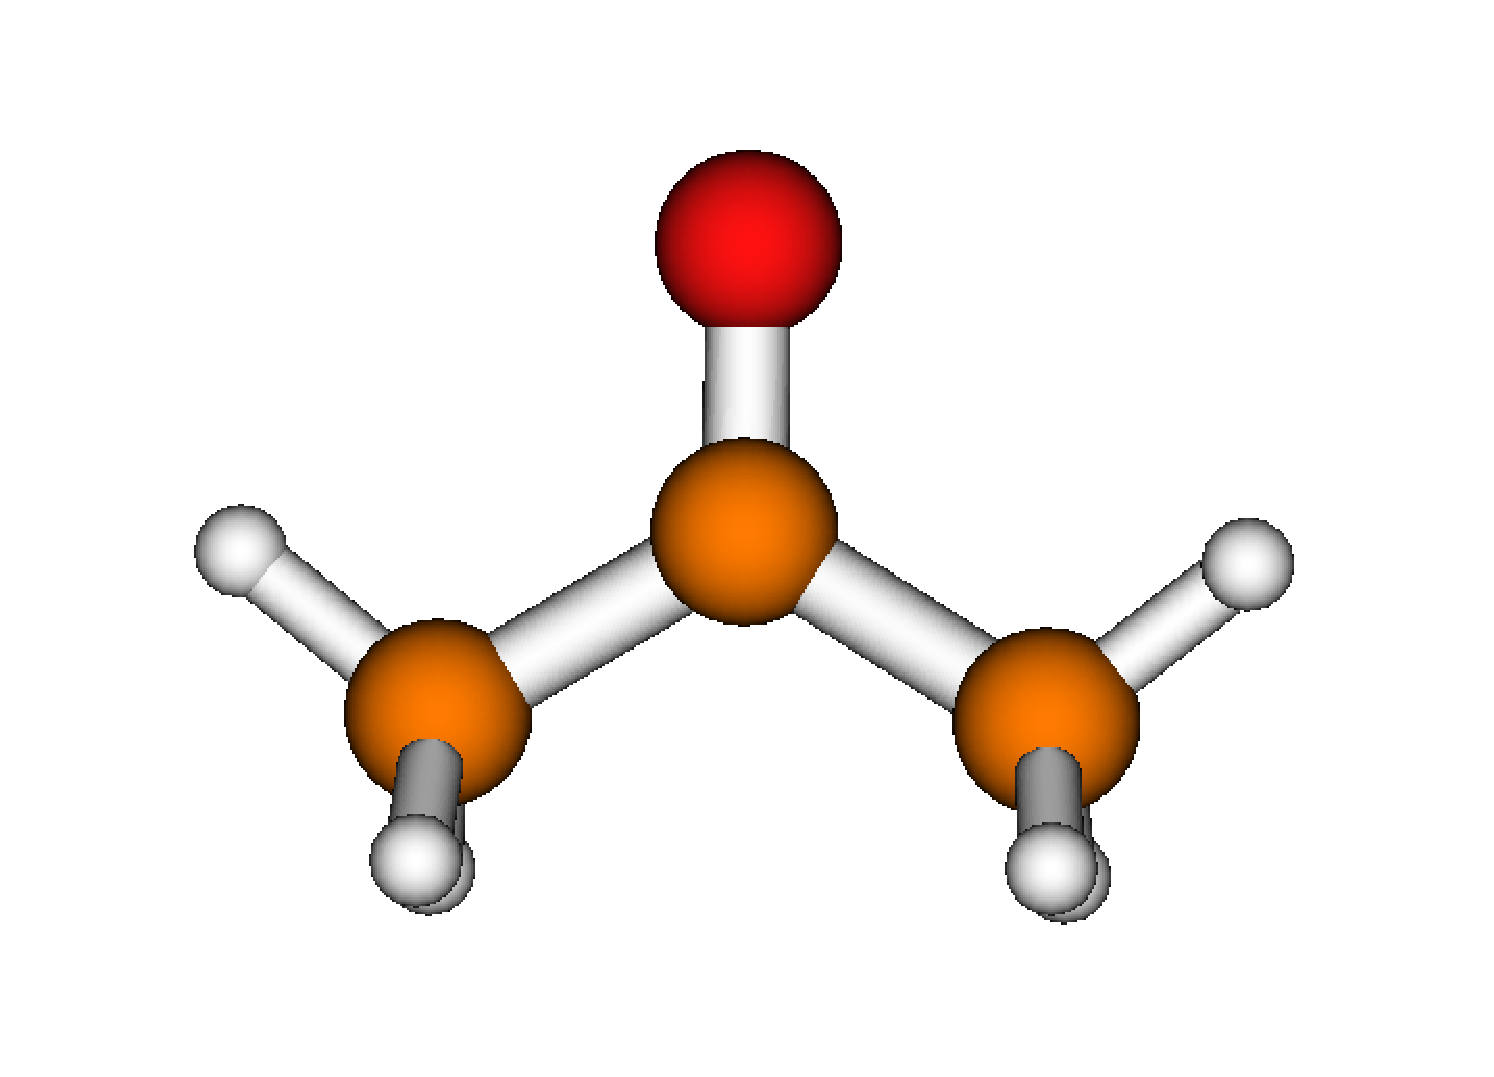
\includegraphics[angle=270,width=7cm,keepaspectratio]{immagini/acetone/geom.eps}
\parbox[h]{12cm}{
\caption{\small Acetone - configurazione spaziale per lo stato fondamentale}
\label{fig:acetone_geom}
}
\end{center}
\end{figure}

L'ottimizzazione di geometria \`e stata effettuata con base 6-311G* a livello CAS,
con uno spazio analogo a quello della formaldeide. La tabella \ref{tab:acetone_geom}
mette a confronto alcuni risultati con il dato sperimentale.
\begin{center}
\begin{threeparttable}
\caption{Acetone - geometria stato fondamentale}
\label{tab:acetone_geom}
\small
\begin{tabular}{|ccc|c|}
\hline
							& CASSCF	& Exp.\tnote{1} \\ 
\hline
$r$(C-O)\tnote{2}			& 1.221		& 1.222				\\
$r$(C-C)\tnote{2}			& 1.511		& 1.507				 \\
$r$(C-H$_1$)\tnote{3}			& 1.081		&			 		 \\
$r$(C-H$_2$)\tnote{3}			& 1.086		&				 	 \\
$\angle$(O-C-C)				& 121.33	& 121.49			 \\
$\angle$(C-C-C)				& 117.33	& 117.02			 \\
\hline
\end{tabular}
\begin{tablenotes}
\parbox[h]{6cm}{
\small
 \item[1] Cfr. \cite{jms-550-551-2000-281}, \cite{jms-120-1986-118} e
 \cite{mp-31-1976-1377}
 \item[] Distanze in Angstroms, angoli in gradi. H$_1$ fa riferimento agli
         idrogeni coplanari al carbonile. H$_2$ agli idrogeni sopra e sotto tale
         piano
}
\end{tablenotes}
\end{threeparttable}
\end{center}
Come si pu\`o notare, la distanza C=O aumenta leggermente, se confrontata
con quella della formaldeide di 1.216 \AA. Ci\`o \`e interpretabile in seguito
all'aumento di interazione sterica tra la nuvola di carica del carbonile e i
gruppi metilici.

La trattazione MCSCF ha richiesto
18 configurazioni, per uno spazio di 6 elettroni in 5 orbitali, illustrati
in figura \ref{fig:acetone_orbitali}. Dal momento che l'acetone possiede la
medesima simmetria della formaldeide, le rappresentazioni irriducibili a cui
apparterranno gli orbitali saranno le medesime elencate in precedenza: A$_1$, B$_1$,
B$_2$ e A$_2$. La distribuzione HF per la molecola di acetone sar\`a quindi
\begin{itemize}
\item 8 di simmetria A$_1$
\item 2 di simmetria B$_1$
\item 5 di simmetria B$_2$
\item 1 di simmetria A$_2$
\end{itemize}

Data la scelta dello spazio CAS, lo spazio inattivo risulta essere
costituito da 7 orbitali di simmetria A$_1$, 1 orbitale di simmetria B$_1$,
4 orbitali di simmetria B$_2$ e 1 orbitale di simmetria A$_2$. Analogamente
al caso della formaldeide, lo stato elettronico finale della transizione
$n_y \rightarrow \pistar$ sar\`a B$_2 \otimes $B$_1 = $A$_2 $.

\begin{figure}[htb]
\begin{center}
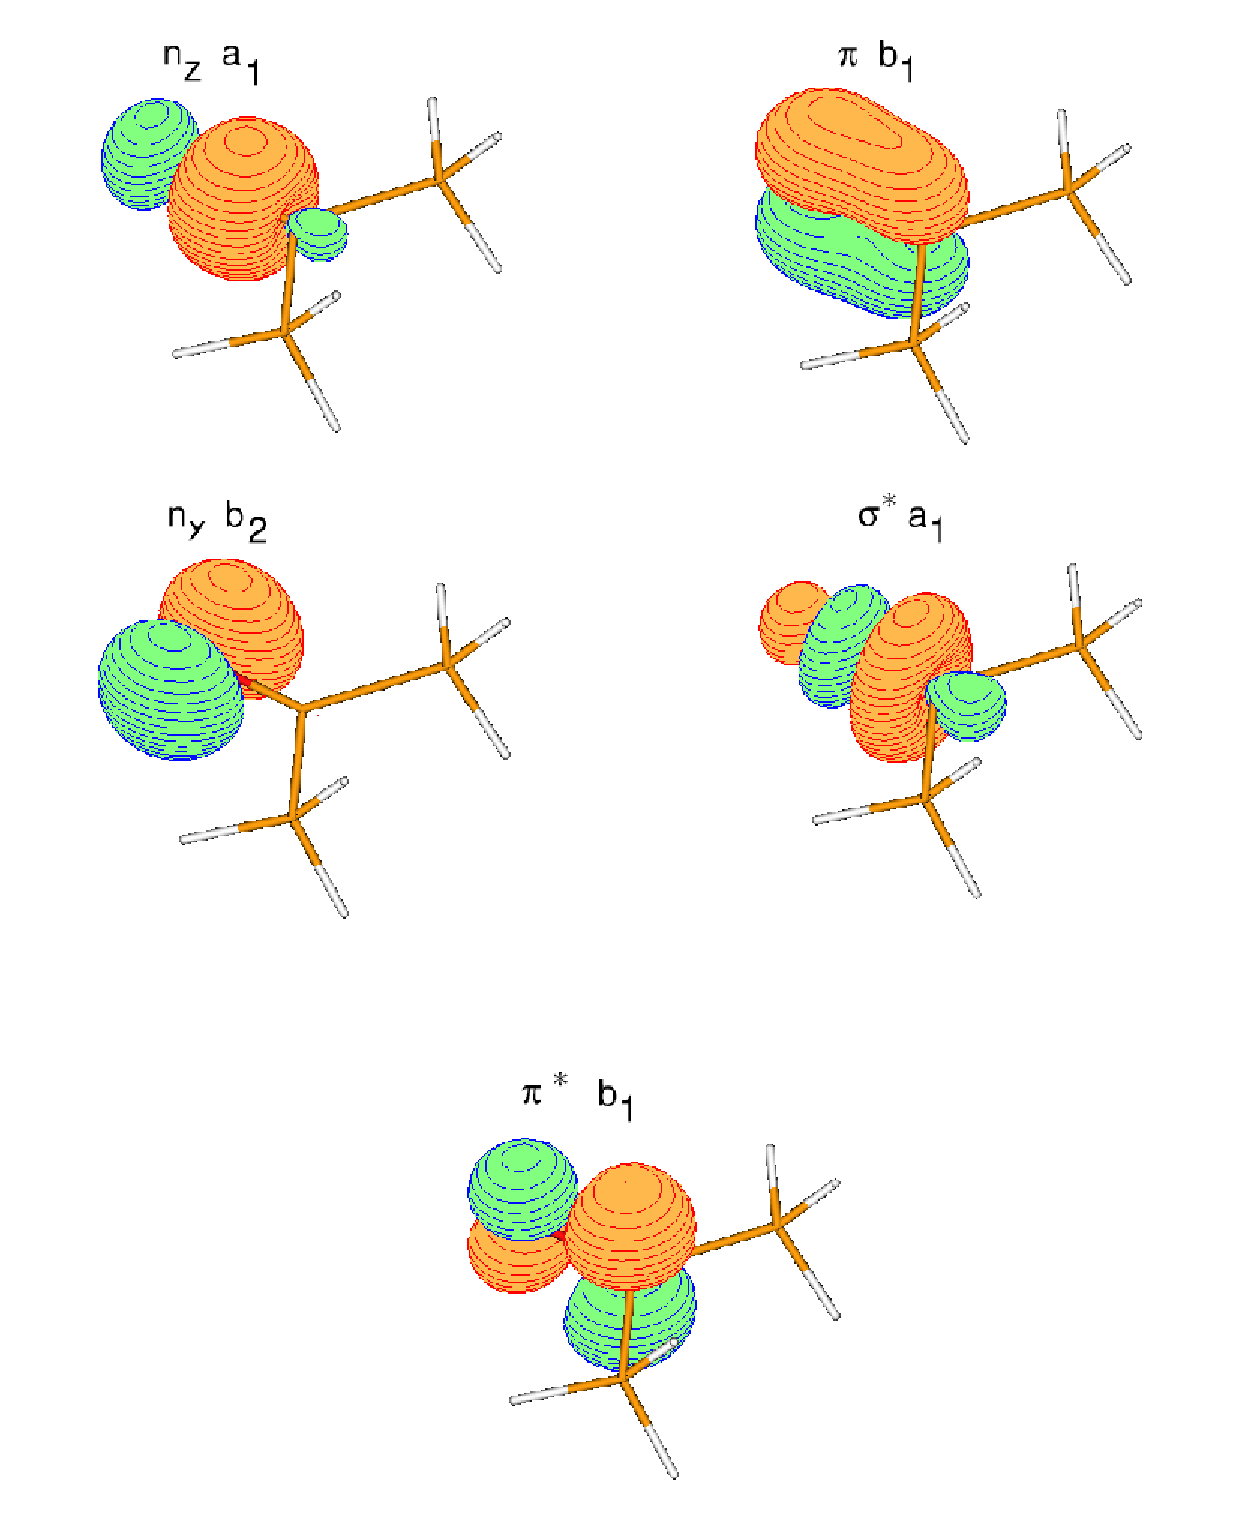
\includegraphics[width=8cm,keepaspectratio]{immagini/acetone/orbitali.eps}
\end{center}
\caption{Spazio CAS per l'acetone}
\label{fig:acetone_orbitali}
\end{figure}

La tabella mostra i numeri di occupazione per lo
stato fondamentale
\begin{verbatim}
 Simmetria A1 : 1.978732113   0.021697330
 Simmetria B1 : 1.938253072   0.062093260 
 Simmetria B2 : 1.999224225
\end{verbatim}

L'energia CASSCF finale per questa base (6-311G*) \`e -192.074240 Hartree.

L'analisi della transizione verticale ha fornito, per lo stato eccitato, un'energia 
-191.895199 Hartree, con una transizione rispetto allo stato fondamentale
di 4.87 eV, contro un valore sperimentale di 4.43 eV (Cfr. \cite{cpl-241-0-1995-26}).
La tabella seguente mostra i numeri di occupazione per lo
stato eccitato
\begin{verbatim}
 Simmetria A1 : 1.984561941   0.015780241 
 Simmetria B1 : 1.996558895   1.003098923
 Simmetria B2 : 1.000000000
\end{verbatim}

Il calcolo effettuato per la transizione adiabatica ha fornito un'energia finale di
-191.932347 Hartree, pari ad una transizione di 3.86 eV contro un valore sperimentale di 3.77 eV
(Cfr. \cite{jcp-111-1-1999-205}). Anche in questo caso, come \`e prevedibile,
il legame carbonilico si allunga in seguito all'occupazione dell'orbitale di
antilegame.
\begin{center}
\begin{threeparttable}
\caption{\small Acetone - geometria di transizione adiabatica}
\label{tab:acetone_geometrie_adiab}
\small
\begin{tabular}{|c|cc|}
\hline
				& CASSCF	& $n_y \rightarrow \pistar$  \\
\hline
$r$(C-O)			& 1.221		& 1.397				\\
$r$(C-C)		& 1.511		& 1.499				 \\
$r$(C-H$_1$)		& 1.080		& 1.084		 		 \\
$r$(C-H$_2$)		& 1.086		& 1.083			 	 \\
$r$(C-H$_3$)		& 1.086		& 1.089			 	 \\
$\angle$(O-C-C)		& 121.33	& 112.13			 \\
$\angle$(C-C-C)		& 117.33	& 121.32			 \\
\hline
\end{tabular}
\begin{tablenotes}
\small
 \item[] Distanze in Angstroms, angoli in gradi
\end{tablenotes}
\end{threeparttable}
\end{center}

\subsubsection{Dipendenza dalla base atomica}

Similmente alla molecola di formaldeide, abbiamo condotto calcoli a
livello CASSCF e perturbativo con le basi
\begin{itemize}
 \item 6-31G
 \item cc-pVDZ
 \item ano-1 (con riduzione 3s2p1d per il carbonio e 2s1p per l'idrogeno)
 \item 6-311G* 
 \item cc-pVTZ
 \item cc-pVQZ
\end{itemize}
i risultati sono mostrati in tabella \ref{tab:acetone_vertical_basis}
\begin{center}
\begin{threeparttable}
\caption{\small Acetone - Energia di transizione $n_y \rightarrow \pistar$ verticale di singoletto, metodi CASSCF e CASSCF/NEV-PT}
\label{tab:acetone_vertical_basis}
{
\small
\begin{tabular}{|c|ccc|ccc|}
\hline
 Base	& \multicolumn{3}{c|}{GS\tnote{1}}				& \multicolumn{3}{c|}{$n_y \rightarrow \pistar$ vert.\tnote{2}} \\
		& CASSCF		& NEV-PT	& NEV-PT	& CASSCF		& NEV-PT & NEV-PT \\
		& 				& SC		& PC		&				& SC 	&	 PC \\
\hline
6-31G	& 0.953869		& 1.263394		& 1.265603		& 4.31			& 4.19		& 4.19		    \\
cc-pVDZ	& 1.048077		& 1.567089		& 1.569608		& 4.84			& 4.50		& 4.50			\\
ano-1	& 1.095777		& 1.612795		& 1.615686 		& 4.87			& 4.54 		& 4.53			\\
6-311G*	& 1.074240		& 1.658429		& 1.660956		& 4.87 			& 4.53		& 4.54 			\\
cc-pVTZ & 1.104413		& 1.810794		& 1.813551		& 4.90			& 4.51 		& 4.51			\\
\hline
\hline
Exp.\tnote{3}	&				& 				&				& \multicolumn{3}{c|}{4.43} \\
\hline
\end{tabular}
}
\begin{tablenotes}
\small
 \item[1] Energia come -(191 + valore) Hartree.
 \item[2] Valori in eV.
 \item[3] Cfr. \cite{cpl-241-0-1995-26}
\end{tablenotes}
\end{threeparttable}
\end{center}

Per quanto riguarda la transizione adiabatica, in tabella \ref{tab:acetone_adiab_basis},
si \`e nuovamente tenuto conto della differenza di ZPE tra lo stato fondamentale e quello eccitato.

\begin{center}
\begin{threeparttable}
\caption{\small Acetone - Energia di transizione $n_y \rightarrow \pistar$ adiabatica di singoletto, metodi CASSCF e CASSCF/NEV-PT}
\label{tab:acetone_adiab_basis}
{
\small
\begin{tabular}{|c|ccc|ccc|}
\hline
Base	& ZPE		& ZPE 			& $\Delta$ZPE	& CASSCF & NEV-PT & NEV-PT \\
		& (GS)		& (Ecc.)		& 				& ZPE 	& SC/ZPE & PC/ZPE \\
\hline
6-31G	& 2.437			& 2.382				& -0.055		&  3.40		 & 3.36 		  & 3.38		\\
cc-pVDZ & 2.402			& 2.350				& -0.052		&  3.81		 & 3.70			  & 3.72		\\
ano-1	& 2.419 		& 2.369				& -0.050		&  3.81 	 & 3.69		  	  & 3.70		\\
6-311G* & 2.414			& 2.367				& -0.047		&  3.81		 & 3.72			  & 3.75		\\
cc-pVTZ & 2.399         & 2.350				& -0.049		&  3.84		 & 3.78		 	  & 3.80		\\
\hline
\hline
Exp.\tnote{1} &				& 					& 				& \multicolumn{3}{c|}{3.77}					\\
\hline
\end{tabular}
}
\begin{tablenotes}
\small
 \item[1] Cfr. \cite{jcp-111-1-1999-205}
 \item[] Valori in eV
\end{tablenotes}
\end{threeparttable}
\end{center}

Nelle figure \ref{fig:acetone_gs}, \ref{fig:acetone_vert} e
\ref{fig:acetone_adiab} sono diagrammate le energie assolute degli stati
fondamentale, eccitato verticale ed eccitato adiabatico rispettivamente,
a livello CASSCF (linea rossa), NEV-PT/SC (linea verde) e NEV-PT/PC
(linea blu).
\begin{figure}[ht]
\begin{center}
\includegraphics[angle=270,width=10cm,keepaspectratio]{immagini/acetone/gs.eps}
\parbox[h]{12cm}{
\caption{\small Acetone - Energia dello stato fondamentale a livello CASSCF (linea rossa),
NEV-PT/SC (linea verde) e NEV-PT/PC (linea blu) come funzione della base
atomica.}
\label{fig:acetone_gs}
}
\end{center}
\end{figure}
\begin{figure}[ht]
\begin{center}
\includegraphics[angle=270,width=10cm,keepaspectratio]{immagini/acetone/vert.eps}
\parbox[h]{12cm}{
\caption{\small Acetone - Energia dello stato eccitato (transizione verticale)
a livello CASSCF (linea rossa), NEV-PT/SC (linea verde) e NEV-PT/PC (linea blu)
come funzione della base atomica. }
\label{fig:acetone_vert}
}
\end{center}
\end{figure}
\begin{figure}[ht]
\begin{center}
\includegraphics[angle=270,width=10cm,keepaspectratio]{immagini/acetone/adiab.eps}
\parbox[h]{12cm}{
\caption{\small Acetone - Energia dello stato eccitato (transizione adiabatica)
a livello CASSCF (linea rossa), NEV-PT/SC (linea verde) e NEV-PT/PC (linea blu)
come funzione della base atomica. }
\label{fig:acetone_adiab}
}
\end{center}
\end{figure}
\pagebreak
\clearpage
Graficando l'energia delle transizioni verticale e adiabatica possiamo notare come
la trattazione perturbativa porti a migliori risultati anche in questo caso.
\begin{figure}[ht]
\begin{center}
\includegraphics[angle=270,width=9cm,keepaspectratio]{immagini/acetone/energie_vert.eps} \\
\includegraphics[angle=270,width=9cm,keepaspectratio]{immagini/acetone/energie_adiab.eps}
\parbox[h]{12cm}{
\caption{\small Acetone - energia di transizione verticale (in alto) e adiabatica (sopra) su basi differenti a livello CASSCF (linea rossa), NEV-PT/SC (linea verde) e NEV-PT/PC (linea blu) come funzione della base atomica.}
\label{fig:acetone_energie_vert_adiab}
}
\end{center}
\end{figure}
\clearpage
%\begin{figure}[ht]
%\begin{center}
%\includegraphics[angle=270,width=6cm,keepaspectratio]{immagini/acetone/energie_adiab.eps}
%\parbox[h]{12cm}{
%\caption{\small Acetone - energia di transizione adiabatica su basi differenti a livello CASSCF (linea rossa), NEV-PT/SC (linea verde) e NEV-PT/PC (linea blu) come funzione della base atomica.}
%\label{fig:acetone_energie_adiab}
%}
%\end{center}
%\end{figure}
%\clearpage

\subsection{Acetaldeide}

Abbiamo successivamente analizzato la molecola di acetaldeide
\begin{figure}[ht]
\begin{center}
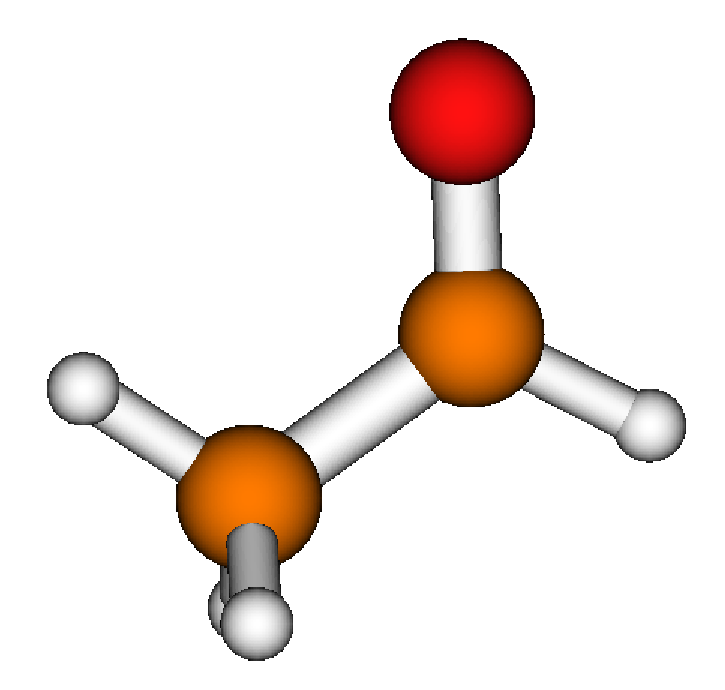
\includegraphics[angle=270,width=7cm,keepaspectratio]{immagini/acetaldeide/geom.eps}
\parbox[h]{10cm}{
\caption{\small Acetaldeide - configurazione spaziale per lo stato fondamentale}
\label{fig:acetaldeide_geom}
}
\end{center}
\end{figure}

Appartenente al gruppo C$_s$, l'acetaldeide ha presentato maggiori
difficolt\`a durante la trattazione richiesta, a causa della ridotta
simmetria rispetto alle molecole precedentemente analizzate. Tale
diversit\`a non consente un perfetto controllo della natura degli orbitali
che definiscono lo spazio CAS: la
selezione degli orbitali gi\`a descritta in precedenza deve ora appartenere
a due sole rappresentazioni irriducibili, la A$^{\prime}$ e la A$^{\prime\prime}$.

Nella tabella dei caratteri qui sotto riportata abbiamo posto l'asse $z$
allineato con il gruppo carbonile, ed il piano $yz$ come elemento di
simmetria per la riflessione \begin{center}
\begin{tabular}{c|cc|c}
  C$_s$				& E		& $\sigma_{yz}$	&           \\
\hline
    A$^{\prime}$  		& 1		&   1			&  $y$, $z$	\\
    A$^{\prime\prime}$	& 1		&  -1			&  $x$      \\
\end{tabular}
\end{center}
In questo modo, \`e possibile interpretare la molecola di acetaldeide, dal
punto di vista della simmetria, in maniera analoga alle molecole viste in
precedenza. Per questa ragione, gli orbitali $\pi$ e $\pistar$ apparterranno alla
rappresentazione irriducibile A$^{\prime\prime}$, in quanto antisimmetrici
rispetto alla riflessione sul piano della molecola, mentre i restanti
orbitali $n_y$, $\sigma$ e $\sigma^{*}$ apparterranno alla rappresentazione
A$^{\prime}$.

Al solito, si \`e scelto uno spazio attivo compatibile alle precedenti
caratterizzazioni e si sono effettuati calcoli sulla base 6-311G* al fine di
ottenere la geometria dello stato fondamentale. 
La scelta ha comportato uno spazio inattivo costituito da 8 orbitali di
simmetria A$^{\prime}$ e 1 orbitale di simmetria A$^{\prime\prime}$, e uno
spazio attivo di 3 orbitali A$^{\prime}$ e 2 orbitali A$^{\prime\prime}$.
Con questa scelta, per descrivere la molecola sono necessarie 28
configurazioni nell'espansione CAS-CI.

La figura \ref{fig:acetaldeide_orbitali_5} mostra gli orbitali dello spazio
attivo per lo stato fondamentale

\begin{figure}[htb]
\caption{\small Spazio CAS per l'acetaldeide}
\label{fig:acetaldeide_orbitali_5}
\begin{center}
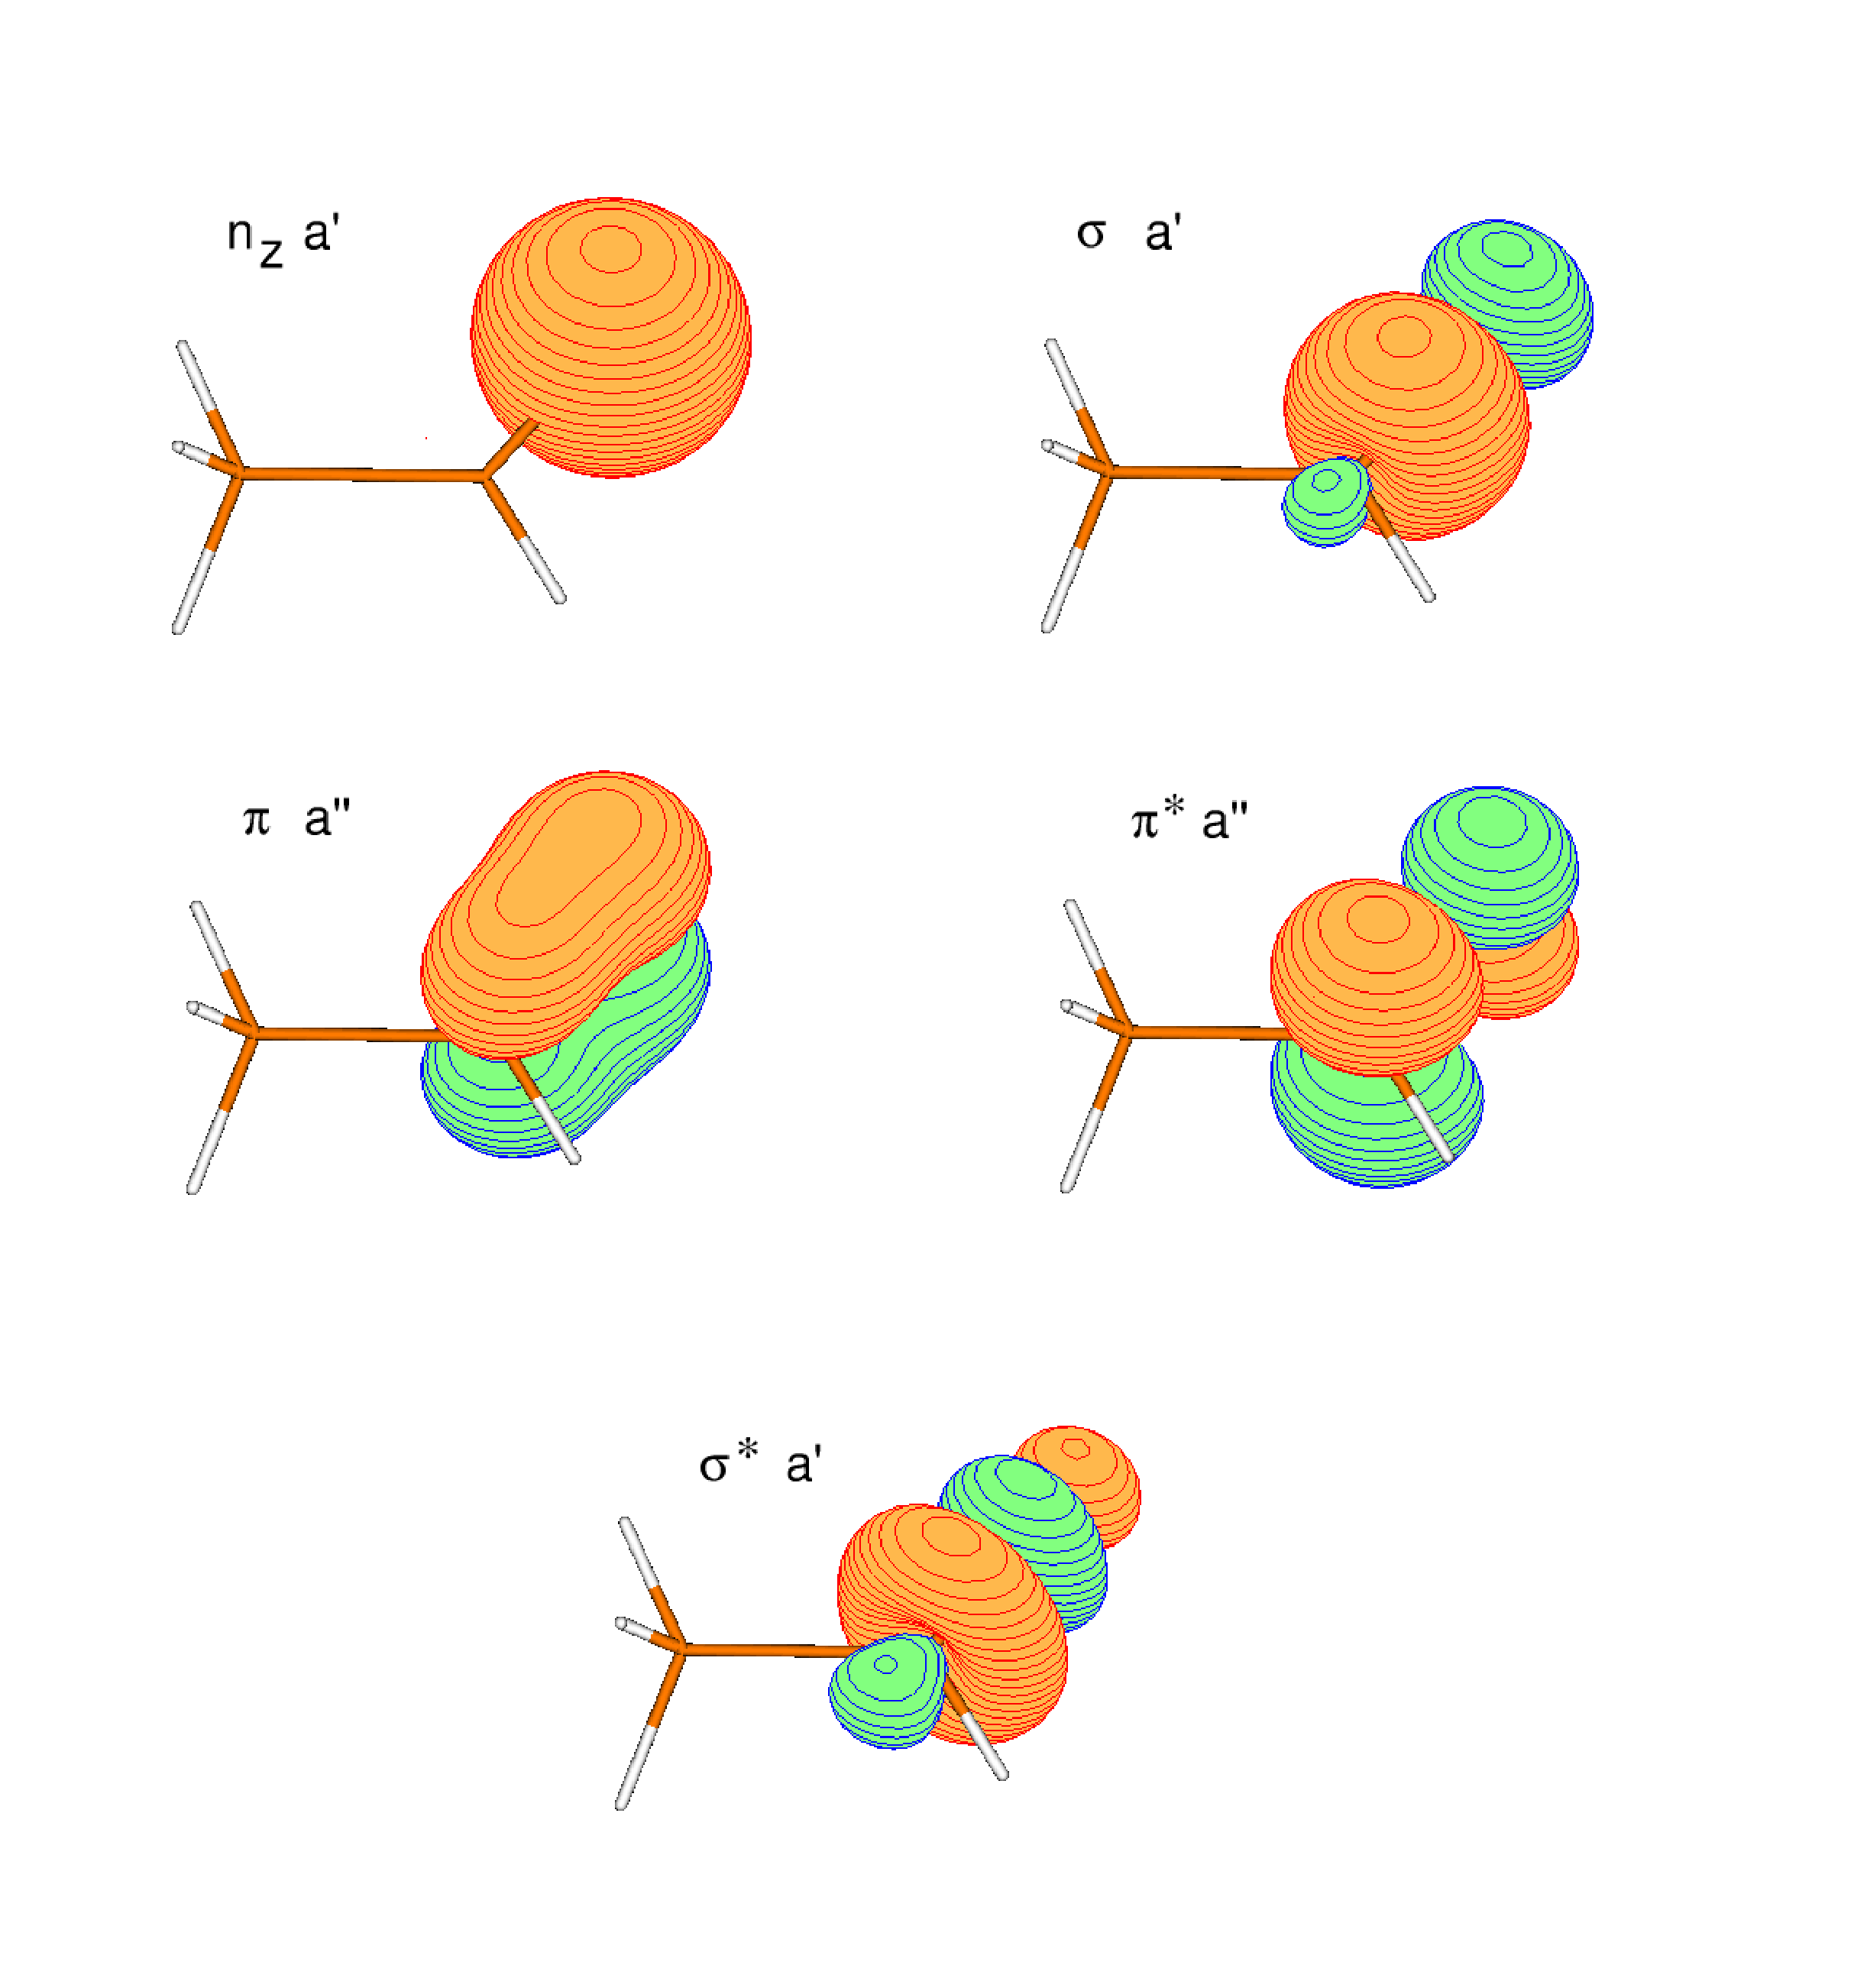
\includegraphics[width=9cm,keepaspectratio]{immagini/acetaldeide/orbitali_5.eps}
\end{center}
\end{figure}

\clearpage
Come \`e possibile notare, lo spazio attivo per lo stato fondamentale
\`e diverso da quello atteso: l'orbitale $n_y$ \`e stato
sostituito dall'orbitale $n_z$.

La ragione di tale variazione \`e imputabile al metodo di convergenza
dell'algoritmo CASSCF, che trova una migliore via di ottimizzazione (con
conseguente maggiore ottimizzazione variazionale dell'energia) attraverso
l'inclusione, nello spazio attivo, dell'orbitale $n_z$ anzich\'e dell'orbitale
$n_y$. Nei casi precedentemente trattati formaldeide e acetone, la simmetria
permetteva un controllo maggiore, in quanto gli orbitali $n_y$ ed $n_z$
appartenevano a rappresentazioni differenti.

Al contrario, lo stato eccitato di simmetria A$^{\prime\prime}$ ha il
corretto spazio attivo, in quanto il maggior contributo correlativo viene
ottenuto includendo gli orbitali interessati al fenomeno, e l'algoritmo
di ricerca del minimo energetico sceglie uno spazio fisicamente corretto.

Come conseguenza di tale errore, l'energia dello stato fondamentale \`e
troppo ottimizzata, perch\'e pi\`u bassa rispetto allo stato contenente
l'orbitale $n_y$ nello spazio attivo. Ne risulta perci\`o un'energia di
eccitazione sia verticale che adiabatica troppo alta.

Sebbene quindi uno spazio attivo cos\`i designato sia errato per questo tipo
di calcolo, la medesima strategia attuata su formaldeide e acetone \`e stata
attuata anche sull'acetaldeide, per meglio valutare come il metodo
perturbativo non sia in grado di porre rimedio ad una intrinseca incorretta
descrizione di uno degli stati di interesse. 
Seguir\`a uno studio ulteriore sulla molecola di
acetaldeide con uno spazio CAS allargato a 5 orbitali A$^{\prime}$ e 2
orbitali A$^{\prime\prime}$, che contenendo interamente la fisica di
interesse dovrebbe fornire, ed in effetti fornisce, risultati sensibilmente
pi\`u accurati.

L'ottimizzazione geometrica, riferita alla disposizione degli atomi mostrata
in figura, ha fornito i dati in tabella \ref{tab:acetaldeide_geom}

\begin{figure}[ht]
\begin{center}
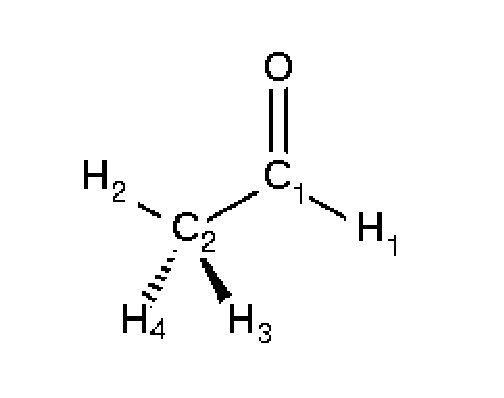
\includegraphics[angle=0,width=44mm,keepaspectratio]{immagini/acetaldeide/2d.eps}
\label{fig:acetaldeide_2d}
\end{center}
\end{figure}

\begin{center}
\begin{threeparttable}
\caption{\small Acetaldeide - geometria per lo stato fondamentale}
\label{tab:acetaldeide_geom}
\small
\begin{tabular}{|l|c|c|}
\hline
								& 6-311G*& Exp.\tnote{1} \\ %& 6-311G*/CAS $n_x \rightarrow \pistar$ \\
								& CAS(6,5)& 	 \\ %& 6-311G*/CAS $n_x \rightarrow \pistar$ \\
\hline
$r$(C$_1$-O)					& 1.21789		& 1.213 	\\%& 1.389869 \\
$r$(C$_1$-C$_2$)				& 1.50284		& 1.504		\\%& 1.497634 \\	
$r$(C$_1$-H$_1$)				& 1.09208		& 1.106		\\%& 1.078165 \\	
$r$(C$_2$-H$_2$)				& 1.08148		& 1.091		\\
$r$(C$_2$-H$_{3/4}$)			& 1.08588		& 1.085		\\
$\angle$(O-C$_1$-C$_2$)			& 124.007		& 124.0		\\%& 114.112 \\	
$\angle$(O-C$_1$-H$_1$)			& 119.395		& 121.1		\\%& 111.097 \\	
$\angle$(C$_2$-C$_1$-H$_1$)		& 116.598		& 114.9		\\%& 120.477 \\	
$\angle$(C$_1$-C$_2$-H$_{3/4}$)	& 110.148		& 110.6		\\%& 		 \\	
$\angle$(C$_1$-C$_2$-H$_2$)		& 110.347		& 110.6		\\%& 		 \\	
$\angle$(H$_3$-C$_2$-H$_4$)		& 107.232	 	&		\\%& 		 \\	
$\angle$(H$_2$-C$_2$-H$_{3/4}$)	& 109.454 		&		\\%& 		 \\	
$\tau$(O-C$_1$-C$_2$-H$_{3/4}$)	& $\pm120.959$	&		\\%& 		 \\	
\hline
\end{tabular}
\begin{tablenotes}
\small
 \item[1] Cfr. \cite{jpc-97-17-1993-4293}
 \item[] Distanze in Angstroms, angoli in gradi.
\end{tablenotes}
\end{threeparttable}
\end{center}

L'energia CASSCF a questa geometria \`e -153.024830 Hartree.
La transizione \mbox{$n_y \rightarrow \pistar$}, di simmetria $A^{\prime\prime}$,
ha energia CASSCF di -152.849283 Hartree. Conseguentemente, l'energia di transizione risulta essere 4.78 eV, contro
un valore sperimentale di 4.28 eV (Cfr. \cite{cpl-241-0-1995-26}).
Nel caso della transizione adiabatica, l'energia dello stato eccitato \`e -152.883379 Hartree, con una energia
di transizione pari a 3.85 eV, contro un valore sperimentale di 3.69 eV (Cfr. \cite{jpc-97-17-1993-4293})
La geometria di tale stato eccitato \`e mostrata in tabella \ref{tab:acetaldeide_geometrie_adiab}

\begin{center}
\begin{threeparttable}
\caption{\small Acetaldeide - geometria per lo stato eccitato adiabatico}
\label{tab:acetaldeide_geometrie_adiab}
\small
\begin{tabular}{|l|c|c|}
\hline
								& GS			&  $n_y \rightarrow \pistar$ \\ 
\hline
$r$($C_1$-O)					& 1.21789		& 1.38987 	\\
$r$($C_1$-$C_2$)				& 1.50284		& 1.49764	\\
$r$($C_1$-$H_1$)				& 1.09208		& 1.07816	\\
$r$($C_2$-$H_2$)				& 1.08148		& 1.08435	\\
$r$($C_2$-$H_3$)				& 1.08588		& 1.08290	\\
$r$($C_2$-$H_4$)				& 1.08588		& 1.08783	\\
$\angle$(O-$C_1$-$C_2$)			& 124.007		& 114.112	\\
$\angle$(O-$C_1$-$H_1$)			& 119.395		& 111.096	\\
$\angle$($C_1$-$C_2$-$H_1$)		& 116.598		& 120.478	\\
$\angle$($C_1$-$C_2$-$H_3$)		& 110.148		& 110.128	\\
$\angle$($C_1$-$C_2$-$H_4$)		& 110.148		& 111.455	\\
$\angle$($C_1$-$C_2$-$H_2$)		& 110.347		& 110.788   \\
$\angle$($H_3$-$C_2$-$H_4$)		& 107.232		& 108.365	\\
$\angle$($H_2$-$C_2$-$H_3$)		& 109.454		& 108.093	\\
$\angle$($H_2$-$C_2$-$H_4$)		& 109.454		& 107.902	\\
$\tau$(O-$C_1$-$C_2$-$H_4$)		& 120.959		&  65.135	\\
$\tau$(O-$C_1$-$C_2$-$H_3$)		& -120.959		& -174.562	\\
$\tau$(O-$C_1$-$C_2$-$H_2$)		& 0.0			& -55.029 	\\
$\tau$($H_2$-$C_2$-$C_1$-$H_1$)	& 180.0			& 168.836 	\\
\hline
\end{tabular}
\begin{tablenotes}
\small
 \item[] Distanze in Angstroms, angoli in gradi.
\end{tablenotes}
\end{threeparttable}
\end{center}
\subsubsection{Perturbazione su uno spazio CAS 6 elettroni/5 orbitali}

La tabella \ref{tab:acetaldeide_vertical_basis_5} presenta i risultati
ottenuti su un CAS con 6 elettroni in 5 orbitali, spazio CAS che, come gi\`a
enunciato, \`e errato in quanto descrive i due stati in modo sbilanciato.

\begin{center}
\begin{threeparttable}
\caption{\small Acetaldeide - Energia di transizione verticale {$n_y \rightarrow \pistar$} di singoletto, CAS 6 elettroni 5 orbitali}
\label{tab:acetaldeide_vertical_basis_5}
\small
\begin{tabular}{|c|ccc|ccc|}
\hline
Basis	& \multicolumn{3}{c|}{GS\tnote{1}}				& \multicolumn{3}{c|}{$n_y \rightarrow \pistar$ vert.\tnote{2}} \\
		& CASSCF		& NEV-PT	 	&	NEV-PT		& CASSCF		& NEV-PT	& NEV-PT  \\
		& 				& SC 			&	PC			& 				& SC		& PC 	 \\
\hline
6-31G	& 0.925561		& 1.143647		&	1.145329	& 4.19			& 4.07 		& 4.06	\\
cc-pVDZ	& 1.002377	 	& 1.380037		&	1.382306	& 4.74			& 4.49 		& 4.49	\\
ano-1	& 1.040915	 	& 1.415777		&	1.418769	& 4.74			& 4.51 		& 4.49	\\
6-311G*	& 1.024830	 	& 1.454798		&	1.457103	& 4.78			& 4.49 		& 4.50	\\
cc-pVTZ & 1.048304	 	& 1.568727		&	1.571395	& 4.78			& 4.48 		& 4.47	\\			
\hline
\hline
Exp.\tnote{3}&				& 				& 				& \multicolumn{3}{c|}{4.28} \\
\hline
\end{tabular}
\begin{tablenotes}
 \item[1] Energia come -(152 + valore) Hartree
 \item[2] Valori in eV
 \item[3] Cfr. \cite{jpc-97-17-1993-4293}
\end{tablenotes}
\end{threeparttable}
\end{center}

Come \`e possibile vedere, nonostante l'applicazione della trattazione
perturbativa, il risultato calcolato \`e ancora distante dal valore
sperimentale. Analogo risultato si ottiene dalla comparazione dei
valori per la transizione adiabatica

\begin{center}
\begin{threeparttable}
\caption{\small Acetaldeide - Energia di transizione adiabatica $n_y \rightarrow \pistar$ di singoletto, CAS 6 elettroni 5 orbitali}
\label{tab:acetaldeide_adiab_basis_5}
\small
\begin{tabular}{|c|ccc|ccc|}
\hline
Basis	& ZPE 			& ZPE 			& $\Delta$ZPE		& CASSCF	& NEV-PT			& NEV-PT  \\
		& 	(GS)		&  (Ecc.) 		& 					& ZPE		& SC/ZPE			& PC/ZPE  \\
\hline
6-31G	& 1.612			& 1.546			& -0.066			& 3.35			& 3.33			& 3.34 \\
cc-pVDZ & 1.593			& 1.534			& -0.059			& 3.78 			& 3.76			& 3.78 \\
ano-1	& 1.603			& 1.545			& -0.058			& 3.78			& 3.75 			& 3.77 \\
6-311G* & 1.600			& 1.545			& -0.055			& 3.79			& 3.78			& 3.80 \\
cc-pVTZ & 1.589			& 1.533			& -0.056			& 3.81			& 3.84			& 3.86 \\
\hline
\hline
Exp.\tnote{1}&				& 				& 					& \multicolumn{3}{c|}{3.69} \\
\hline
\end{tabular}
\begin{tablenotes}
 \item[1] Cfr. \cite{jpc-97-17-1993-4293}
 \item[ ] Valori in eV
\end{tablenotes}
\end{threeparttable}
\end{center}

Diagrammando le energie di transizione per questo caso, risulta ancora pi\`u
evidente come l'errore rispetto al dato sperimentale sia elevato, sia per la
transizione verticale che per quella adiabatica.

\begin{figure}[ht]
\begin{center}
\includegraphics[angle=270,width=10cm,keepaspectratio]{immagini/acetaldeide/energie_vert_5.eps} \\
\includegraphics[angle=270,width=10cm,keepaspectratio]{immagini/acetaldeide/energie_adiab_5.eps}
\parbox[h]{12cm}{
\caption{\small Acetaldeide - energia di transizione verticale (in alto) ed adiabatica (sopra) su basi differenti a livello CASSCF (linea rossa), NEV-PT/SC (linea verde) e NEV-PT/PC (linea blu) come funzione della base atomica.}
\label{fig:acetaldeide_energie_vert_5}
}
\end{center}
\end{figure}
\clearpage

\`E inoltre evidente come la trattazione perturbativa NEV-PT non riesca ad
effettuare una correzione significativa, in quanto lo scarto rispetto allo
sperimentale \`e causato da una differente natura fisica dello stato
fondamentale, sul quale la trattazione perturbativa non pu\`o recuperare.


\subsection{Acetaldeide - CAS 10 elettroni / 7 orbitali}

Al fine di migliorare la trattazione sull'acetaldeide, si \`e quindi scelto
uno spazio attivo compatibile con la necessit\`a di includere il doppietto $n_y$
sia nello stato fondamentale che nello stato eccitato.

La scelta ha portato ad ampliare lo spazio attivo, fino ad avere
5 orbitali A$^{\prime}$ e 2 orbitali A$^{\prime\prime}$,
e uno spazio di core costituito da 6 orbitali di simmetria A$^{\prime}$
e 1 orbitale di simmetria A$^{\prime\prime}$.
Con questa definizione, sono necessarie 106 configurazioni
nell'espansione CAS-CI, contro le 28 del precedente spazio attivo.

I risultati ottenuti sono rappresentati in tabella \ref{tab:acetaldeide_vertical_basis_7}
\begin{center}
\begin{threeparttable}
\caption{\small Acetaldeide - Energia di transizione verticale $n_y \rightarrow \pistar$ di singoletto, CAS 10 elettroni 7 orbitali}
\label{tab:acetaldeide_vertical_basis_7}
\small
\begin{tabular}{|c|ccc|ccc|}
\hline
Basis	& \multicolumn{3}{c|}{GS\tnote{1}}				& \multicolumn{3}{c|}{$n_y \rightarrow \pistar$ vert.\tnote{2}} \\
		& CASSCF		& NEV-PT	 	&	NEV-PT		& CASSCF		& NEV-PT	& NEV-PT	  \\
		& 				& SC 			&	PC			& 				& SC		& PC	 	 \\
\hline
6-31G	& 0.927916		& 1.138181		&	1.140489	& 4.06			& 4.01		& 4.03		\\
cc-pVDZ	& 1.004396		& 1.370583		&	1.373364	& 4.58			& 4.37		& 4.38		\\
ano-1	& 1.042885		& 1.405010		&	1.408962	& 4.59			& 4.35 		& 4.34		\\
6-311G*	& 1.026837		& 1.445053		&	1.447570	& 4.62			& 4.35		& 4.37		\\
cc-pVTZ & 1.050199		& 1.556482		&	1.559922	& 4.62			& 4.32		& 4.32		\\			
\hline
\hline
Exp.\tnote{3}&				& 				& 				& \multicolumn{3}{c|}{4.28} \\
\hline
\end{tabular}
\begin{tablenotes}
 \item[1] Energia come -(152 + valore) Hartree
 \item[2] Valori in eV
 \item[3] Cfr. \cite{jpc-97-17-1993-4293}
\end{tablenotes}
\end{threeparttable}
\end{center}

\`E evidente come, con uno spazio attivo allargato, si venga incontro alla
necessit\`a fisica di descrivere lo stato fondamentale e quello eccitato
nello stesso modo. I valori per la transizione a livello CAS restano
tuttavia relativamente distanti dal valore vero di 4.28 eV, nonostante il
numero di configurazioni sia considerevolmente aumentato. La perturbazione
consente di recuperare parte dell'energia di correlazione ed avvicinarsi
cos\`i in modo pi\`u deciso all'energia di transizione sperimentale.

Analoghe considerazioni per quanto riguarda la transizione adiabatica,
i cui risultati sono riportati in tabella \ref{tab:acetaldeide_adiab_basis_7}

\begin{center}
\begin{threeparttable}
\caption{\small Acetaldeide - Energia di transizione adiabatica $n_y \rightarrow \pistar$ di singoletto, CAS 10 elettroni 7 orbitali}
\label{tab:acetaldeide_adiab_basis_7}
\small
\begin{tabular}{|c|ccc|ccc|}
\hline
Basis	& ZPE 			& ZPE 			& $\Delta$ZPE		& CASSCF		& NEV-PT		& NEV-PT	 \\
		& (GS)			& (Ecc.) 		& 					& ZPE			& SC/ZPE		& PC/ZPE 	 \\
\hline
6-31G	& 1.612			& 1.544			& -0.068			& 3.32			& 3.30			& 3.33			 \\
cc-pVDZ & 1.592			& 1.531			& -0.062			& 3.73 			& 3.64			& 3.66			 \\
ano-1	& 1.603			& 1.542			& -0.060			& 3.73			& 3.60 			& 3.61			 \\
6-311G* & 1.600 		& 1.543			& -0.057			& 3.74			& 3.65			& 3.66			 \\
cc-pVTZ & 1.590			& 1.531			& -0.059			& 3.76			& 3.68			& 3.69			 \\
\hline
\hline
Exp.\tnote{1}&				& 				& 					& \multicolumn{3}{c|}{3.69} \\
\hline
\end{tabular}
\begin{tablenotes}
 \item[1] Cfr. \cite{jpc-97-17-1993-4293}
 \item[] Valori in eV
\end{tablenotes}
\end{threeparttable}
\end{center}

Come si pu\`o vedere, c'\`e un ottimo accordo tra il dato sperimentale e il
valore calcolato, gi\`a buono a livello CAS, che viene migliorato ulteriormente
dall'applicazione della perturbazione.

Al solito, i grafici \ref{fig:acetaldeide_energie_vert_7} e \ref{fig:acetaldeide_energie_adiab_7}
mostrano l'andamento dei dati sopra rappresentati, permettendo di
evidenziare in modo pi\`u netto l'andamento delle energie di transizione
verticale e adiabatica
\begin{figure}[ht]
\begin{center}
\includegraphics[angle=270,width=11cm,keepaspectratio]{immagini/acetaldeide/energie_vert_7.eps}
\parbox[h]{12cm}{
\caption{\small Acetaldeide - energia di transizione verticale su basi differenti a livello CASSCF (linea rossa), NEV-PT/SC (linea verde) e NEV-PT/PC (linea blu) come funzione della base atomica.}
\label{fig:acetaldeide_energie_vert_7}
}
\end{center}
\end{figure}
\pagebreak
\begin{figure}[ht]
\begin{center}
\includegraphics[angle=270,width=12cm,keepaspectratio]{immagini/acetaldeide/energie_adiab_7.eps}
\parbox[h]{12cm}{
\caption{\small Acetaldeide - energia di transizione adiabatica su basi differenti a livello CASSCF (linea rossa), NEV-PT/SC (linea verde) e NEV-PT/PC (linea blu) come funzione della base atomica.}
\label{fig:acetaldeide_energie_adiab_7}
}
\end{center}
\end{figure}

\clearpage


\section{Sistemi coniugati ciclici}

Lo studio degli stati eccitati \`e proseguito con un'analisi 
delle molecole coniugate cicliche di benzene e naftalene, con
diverse basi orbitaliche.

\subsection{Benzene}

La molecola di benzene, di simmetria D$_{6h}$ \`e stata caratterizzata nello
stato fondamentale e negli stati eccitati di singoletto appartenenti alle rappresentazioni
B$_{2u}$ e B$_{1u}$. A causa di imposizioni del programma \texttt{dalton},
si \`e lavorato con il sottogruppo D$_{2h}$.

Inizialmente si \`e condotto un calcolo esplorativo, su base 6-31G* con spazio
CAS 6/6 definito dagli orbitali $\pi$ e dai corrispondenti $\pistar$. Tale
calcolo ha fornito geometrie e valutazioni degli orbitali e delle loro
simmetrie.

In seguito, per affinare i risultati, si \`e provveduto ad effettuare altre
valutazioni, passando quindi alla base ano-1 definita 3s2p1d per il carbonio
e 2s1p per l'idrogeno, sia con il medesimo spazio CAS sopra descritto, sia
con uno spazio CAS ampliato, ottenuto raddoppiando gli orbitali per ogni
simmetria, e passando di conseguenza ad un CAS 6/12.

La molecola \`e stata posta sul piano $xy$, con l'asse principale orientato
lungo l'asse $z$.

I ben noti orbitali $\pi$ del benzene, orbitali che faranno parte dello
spazio attivo non espanso, in simmetria D$_{6h}$ sono assegnabili alle
rappresentazioni A$_{2u}$, E$_{1g}$, E$_{2u}$ e B$_{2g}$. In simmetria
D$_{2h}$ tali rappresentazioni si trasformano, rispettivamente e ricordando
che le rappresentazioni E sono bidimensionali, in B$_{1u}$, B$_{2g}$,
B$_{3g}$, B$_{1u}$, A$_{u}$ e B$_{2g}$. Gli orbitali appartenenti alle prime
tre rappresentazioni sono occupati.
Sempre in seguito alla diminuzione di simmetria, gli stati eccitati su cui
verranno effettuate valutazioni apparterranno, in simmetria D$_{2h}$,
alle rappresentazioni B$_{2u}$ e B$_{3u}$, anzich\'e B$_{2u}$ e B$_{1u}$,
rispettivamente, per la simmetria D$_{6h}$.

Le geometrie molecolari sono state ottimizzate nelle varie condizioni
operative. Nella tabella \ref{tab:benzene_geom} sono messe a confronto le
geometrie ottenute per via teorica con il dato sperimentale
\begin{center}
\begin{threeparttable}
\caption{\small Benzene - geometrie su diversi metodi/basi}
\label{tab:benzene_geom}
\small
\begin{tabular}{|l|c|c|}
\hline
							& R$_{CC}$		& R$_{CH}$ \\ 
\hline
CASSCF 6/6 / 6-31G*			& 1.396			&	1.075	 \\
CASSCF 6/6 / ano-1			& 1.398			&	1.080	 \\
CASSCF 6/12 / ano-1			& 1.398			&	1.081    \\
Exp.\tnote{1}				& 1.390			&	1.086    \\
\hline
\end{tabular}
\begin{tablenotes}
\small
 \item[1] Cfr. \cite{jms-148-1991-427}
 \item[] Valori in Angstroms
\end{tablenotes}
\end{threeparttable}
\end{center}

\subsubsection{Eccitazione B$_{2u}$ (B$_{2u}$ in D$_{2h}$)}

La transizione elettronica B$_{2u}$ \`e quella a minore energia. Analisi
sperimentali (Cfr. \cite{jcp-94-12-1991-7700}) forniscono per questa
transizione un valore di 4.90 eV, anche se in realt\`a lo spettro in fase gas
e jet-cooled forniscono un inviluppo vibrazionale che va da 4.79 eV
(transizione 0-0) fino a 5.35 eV, con un picco di massimo assorbimento
proprio a 4.90 eV, scelto come riferimento per la transizione Franck-Condon.

La tabella \ref{tab:benzene_b2u} mostra i risultati ottenuti con la
trattazione effettuata.
\begin{center}
\begin{threeparttable}
\caption{\small Benzene - Energia della transizione di singoletto B$_{2u}$
(B$_{2u}$ in D$_{2h}$)}
\label{tab:benzene_b2u}
{
\small
\begin{tabular}{|c|ccc|ccc|}
\hline
 				& \multicolumn{3}{c|}{GS\tnote{1}}				& \multicolumn{3}{c|}{Ecc. B$_{2u}$\tnote{2}} \\
				& CASSCF	& NEV-PT	& NEV-PT	& CASSCF		& NEV-PT	& NEV-PT \\
				&			& SC		& PC		& 				& SC		& PC \\
\hline
CAS(6,6)/6-31G*	& 0.775778	& 1.468765	& 1.469361	& 4.99			& 5.33		& 5.31		\\
CAS(6,6)/ano-1	& 0.830416	& 1.558968	& 1.559728	& 4.92			& 5.22		& 5.20		\\
CAS(6,12)/ano-1	& 0.844274	& 1.558662	& 1.564030	& 4.92			& 5.17		& 5.19		\\
\hline
\hline
Exp.\tnote{3}	&				& 				&				& \multicolumn{3}{c|}{4.90} \\
\hline
\end{tabular}
}
\begin{tablenotes}
\small
 \item[1] Energia come \mbox{-(230 + valore)} Hartree
 \item[2] Valori in eV
 \item[3] Cfr. \cite{jcp-94-12-1991-7700}
\end{tablenotes}
\end{threeparttable}
\end{center}

Apparentemente quindi, il risultato CASSCF \`e in buon accordo con il dato
sperimentale, e la trattazione perturbativa attua un allontanamento dal
valore esatto. Tuttavia, la Ref. \cite{jcp-112-6-2000-2798} sottolinea come
la differenza tra la transizione 0-0 ed il massimo della banda sia 0.19 eV,
mentre sui valori calcolati la differenza tra la transizione 0-0 e la
verticale \`e di 0.31 eV. Di conseguenza, il massimo della banda \`e spostato
di 0.12 eV pi\`u in basso rispetto all'energia verticale Franck-Condon.
Questo implica che il valore sperimentale di 4.90 eV comporta, per la
transizione verticale, un posizionamento a 5.02 eV, in migliore accordo
con i dati ottenuti a livello perturbativo.

\subsubsection{Eccitazione B$_{1u}$ (B$_{3u}$ in D$_{2h}$)}

La transizione B$_{1u}$ viene stimata attorno ai 6.20 eV (Cfr.
\cite{jcp-112-6-2000-2798} e \cite{tca-91-1995-91}). La tabella
\ref{tab:benzene_b1u} mostra i dati ottenuti
\begin{center}
\begin{threeparttable}
\caption{\small Benzene - Energia della transizione di simmetria B$_{1u}$
(B$_{3u}$ in D$_{2h}$)}
\label{tab:benzene_b1u}
{
\small
\begin{tabular}{|c|ccc|}
\hline
 				& \multicolumn{3}{c|}{ Ecc. B$_{1u}$\tnote{2}} \\
				& CASSCF		& NEV-PT/SC & NEV-PT/PC \\
\hline
CAS(6,6)/6-31G*	&  8.18			& 6.75		& 6.71		\\
CAS(6,6)/ano-1	&  7.87			& 6.33 		& 6.26		\\
CAS(6,12)/ano-1	&  7.46			& 6.54		& 6.50		\\
\hline
\hline
Exp.\tnote{3}	&	 \multicolumn{3}{c|}{6.20} \\
\hline
\end{tabular}
}
\begin{tablenotes}
\small
 \item[1] Valori in Hartree
 \item[2] Valori in eV
 \item[3] Cfr. \cite{jcp-112-6-2000-2798} e \cite{tca-91-1995-91}
\end{tablenotes}
\end{threeparttable}
\end{center}

\subsection{Naftalene}

Analoga trattazione \`e stata eseguita sul naftalene, molecola di simmetria
D$_{2h}$.
La molecola \`e stata orientata sul piano $xy$, con l'asse C$_2$ ortogonale al
piano molecolare lungo l'asse $z$.
Il calcolo \`e stato eseguito con base 6-31G* con spazio CAS 10 elettroni in
10 orbitali $\pi$ (per un totale di 4936 configurazioni) e successivamente
con base ano-1 definita 3s2p1d per il carbonio e 2s1p per l'idrogeno. Gli
orbitali facenti parte dello spazio attivo sono caratterizzati dalle
simmetrie B$_{1u}$, B$_{2g}$, B$_{3g}$, B$_{1u}$, A$_u$, B$_{2g}$, B$_{3g}$,
B$_{1u}$, A$_u$ e B$_{3g}$.  A livello HF, solo i primi 5 orbitali
(b$_{1u}$, b$_{2g}$, b$_{3g}$, b$_{1u}$, a$_u$) sono occupati.

La geometria \`e stata ottimizzata su entrambe le basi. Data l'assegnazione
per i legami data in figura

\begin{figure}[ht]
\begin{center}
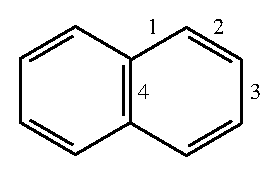
\includegraphics[angle=0,width=4cm,keepaspectratio]{immagini/naftalene/geom.eps}
\end{center}
\end{figure}

i risultati, confrontati con il valore sperimentale (Cfr. \cite{prsls-258-1960-270})
sono visibili in tabella \ref{tab:naftalene_geom}
\begin{center}
\begin{threeparttable}
\caption{\small Naftalene - geometrie su diverse basi}
\label{tab:naftalene_geom}
\small
\begin{tabular}{|l|c|c|c|}
\hline
					& 6-31G*	& ano-1		&	Exp.\tnote{1}	\\ 
\hline
$r_1$				& 1.427		& 1.427		&	1.421	\\
$r_2$				& 1.373		& 1.375		&	1.364	\\
$r_3$				& 1.421		& 1.424		&	1.415	\\
$r_4$				& 1.416		& 1.415		&	1.418	\\
\hline
\end{tabular}
\begin{tablenotes}
\small
 \item[1] Cfr. \cite{prsls-258-1960-270}
 \item[] Valori in Angstroms
\end{tablenotes}
\end{threeparttable}
\end{center}

\subsubsection{Eccitazione B$_{3u}$}

La transizione elettronica che origina lo stato eccitato di simmetria
B$_{3u}$ risulta essere quella con minima energia. Il valore sperimentale
(Cfr. \cite{cpl-16-1972-464} e \cite{jms-26-1968-67}) \`e assegnato a 4.0 eV.

La tabella \ref{tab:naftalene_b3u} mostra i risultati ottenuti con la
trattazione effettuata. Come si vede, I risultati risentono di un certo
errore rispetto al valore sperimentale.
\begin{center}
\begin{threeparttable}
\caption{\small Naftalene - Energia della transizione di simmetria B$_{3u}$. CAS
10/10 su basi differenti}
\label{tab:naftalene_b3u}
{
\begin{tabular}{|c|ccc|ccc|}
\hline
\small
 				& \multicolumn{3}{c|}{GS\tnote{1}}				& \multicolumn{3}{c|}{Ecc. B$_{3u}$\tnote{2}} \\
				& CASSCF		& NEV-PT		& NEV-PT		& CASSCF		& NEV-PT	& NEV-PT \\
				&				& SC			& PC			& 				& SC		& PC	 \\
\hline
6-31G*			& 0.477577		& 1.629822		& 1.631355		& 4.32			& 4.54		& 4.52	\\
ano-1			& 0.565924		& 1.776676		& 1.778645		& 4.29			& 4.46		& 4.43	\\
\hline
\hline
Exp.\tnote{3}	&				& 				&				& \multicolumn{3}{c|}{4.0} \\
\hline
\end{tabular}
}
\begin{tablenotes}
\small
 \item[1] Energia come \mbox{-(383 + valore)} Hartree
 \item[2] Valori in eV
 \item[3] Cfr. \cite{cpl-16-1972-464} e \cite{jms-26-1968-67}
\end{tablenotes}
\end{threeparttable}
\end{center}


\subsubsection{Eccitazione B$_{2u}$}

Per quanto riguarda l'eccitazione B$_{2u}$, i risultati sono decisamente
migliori. A livello CASSCF l'errore \`e elevato, pi\`u di 2 eV. L'applicazione
della perturbazione porta a risultati praticamente coincidenti con il range
accertato per lo sperimentale.

\begin{center}
\begin{threeparttable}
\caption{\small Naftalene - Energia della transizione di simmetria B$_{2u}$}
\label{tab:naftalene_b2u}
{
\small
\begin{tabular}{|c|ccc|}
\hline
 				& \multicolumn{3}{c|}{ Ecc. B$_{2u}$ \tnote{2}} \\
				& CASSCF		& NEV-PT & NEV-PT \\
				& 				& SC	 & PC \\
\hline
6-31G*	&  6.62			& 4.88	 &  4.82 \\
ano-1	&  6.42			& 4.51	 & 4.42	\\
\hline
\hline
Exp.\tnote{3} &	 \multicolumn{3}{c|}{4.45-4.7} \\
\hline
\end{tabular}
}
\begin{tablenotes}
\small
 \item[1] Valori in Hartree
 \item[2] Valori in eV
 \item[3] Cfr. \cite{cpl-16-1972-464}, \cite{jms-26-1968-67} e \cite{jpb-25-1992-2197}
\end{tablenotes}
\end{threeparttable}
\end{center}


\section{Sistemi coniugati lineari}

Per ultimo, lo studio di sistemi coniugati lineari si \`e invece concentrato
sull'esatriene, previa caratterizzazione analoga sull'omologo inferiore
minimale etilene che, pur non essendo a rigore un sistema coniugato, ha
consentito la valutazione essenziale dei parametri e dei risultati in
studio: si \`e valutata la superficie di potenziale per lo stato
fondamentale, definita sui due gradi di libert\`a della rotazione del doppio
legame centrale e della posizione degli idrogeni interessati a tale
rotazione. 

Successivamente, sul sistema esatriene si \`e studiato il percorso di minima
energia (Minimum Energy Path, MEP) e le energie di eccitazione verticale ed
adiabatica, e la conseguente trattazione perturbativa.

\subsection{Etilene}

L'etilene \`e stato scelto quale composto di riferimento per la descrizione
della superficie di potenziale descritta dai gradi di libert\`a di interesse.
Per descrivere la molecola si \`e fatto uso della base 6-31G*, con un CAS 2/2
comprendente gli orbitali $\pi$ e $\pistar$

\begin{figure}[ht]
\begin{center}
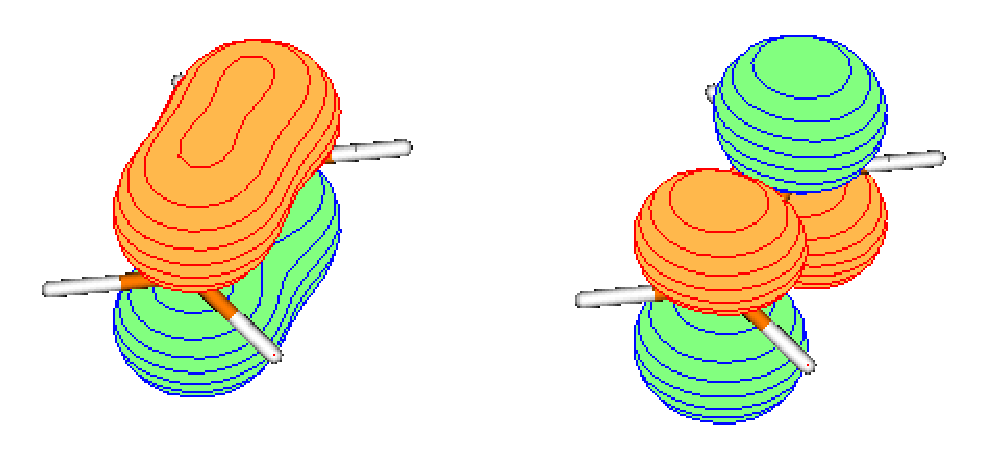
\includegraphics[angle=0,width=7cm,keepaspectratio]{immagini/etene/orbitali.eps}
\parbox[h]{10cm}{
\caption{\small Etilene - orbitali $\pi$ e $\pistar$}
\label{fig:etene_orbitali}
}
\end{center}
\end{figure}

I parametri geometrici in condizioni di equilibrio sono rappresentati in
tabella \ref{tab:etene_geom}, confrontati con un calcolo CASSCF
2/11 con base 6-311(2+)G* (Cfr . \cite{jcp-105-20-1996-9007})
\begin{center}
\begin{threeparttable}
\caption{\small Etilene - geometria per lo stato fondamentale}
\label{tab:etene_geom}
\small
\begin{tabular}{|ccc|c|}
\hline
							& GS		& GS CAS 2/11\tnote{1} \\ 
\hline
$r$(C-C)					& 1.338		& 1.338	\\
$r$(C-H)					& 1.076		& 1.076	 \\
$\angle$(H-C-C)				& 121.7		& 121.7	 \\
\hline
\end{tabular}
\begin{tablenotes}
\small
 \item[1] Cfr. \cite{jcp-105-20-1996-9007}
\end{tablenotes}
\end{threeparttable}
\end{center}

Facendo riferimento alla disposizione degli atomi data in figura
\begin{figure}[ht]
\begin{center}
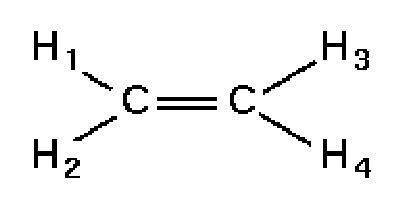
\includegraphics[angle=0,width=3cm,keepaspectratio]{immagini/etene/etene.eps}
\end{center}
\end{figure}
e assumendo che con angolo diedro A-B-C-D si intende l'angolo formato dai
piani definiti da A,B,C e B,C,D, la rotazione attorno al doppio legame 
viene studiata vincolando le torsioni H$_1$-C-C-H$_3$ e H$_2$-C-C-H$_4$, 
modificandone il valore da $0^{\circ}$ a $180^{\circ}$, ed eseguendo
l'ottimizzazione geometrica sui restanti gradi di libert\`a. Ne risulta
la superficie di potenziale, mostrata in figura \ref{fig:etene_3d}.

\begin{figure}[ht]
\begin{center}
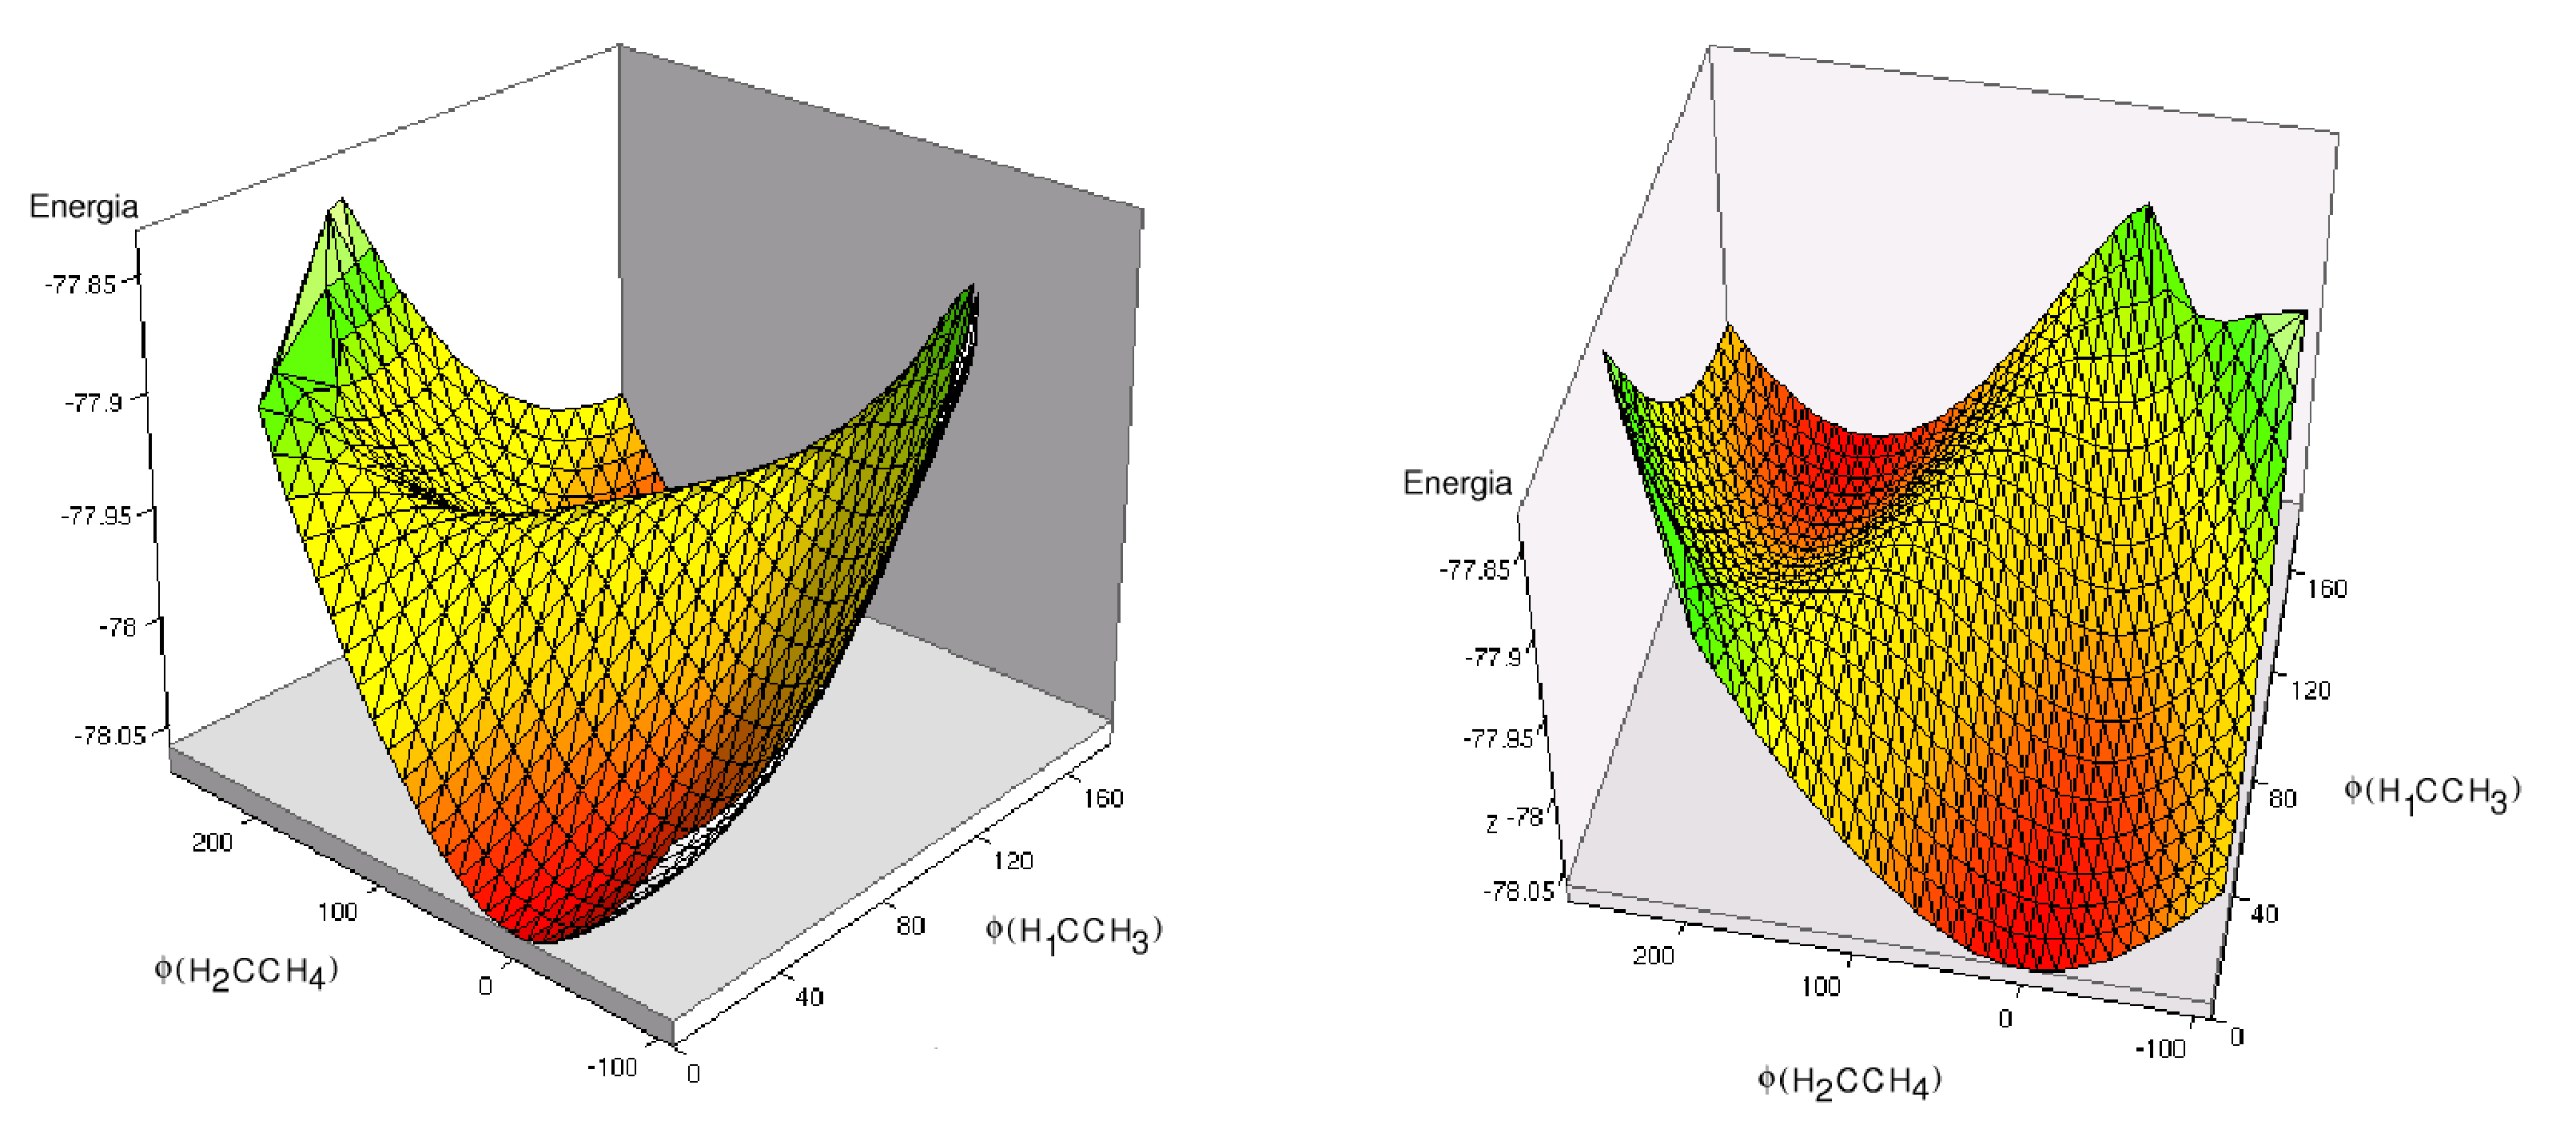
\includegraphics[angle=0,width=12cm,keepaspectratio]{immagini/etene/3d.eps}
\caption{\small Etilene - superfici di potenziale}
\label{fig:etene_3d}
\end{center}
\end{figure}

\`E possibile notare come tale superficie presenti due valli parallele,
ciascuna delle quali degenera in una spalla quando l'energia del minimo
diviene eccessivamente elevata. Una sezione della superficie a 
H$_1$-C-C-H$_3$ pari a 90$^{\circ}$ mostra un doppio minimo, con energie comparabili. 
\begin{figure}[ht]
\begin{center}
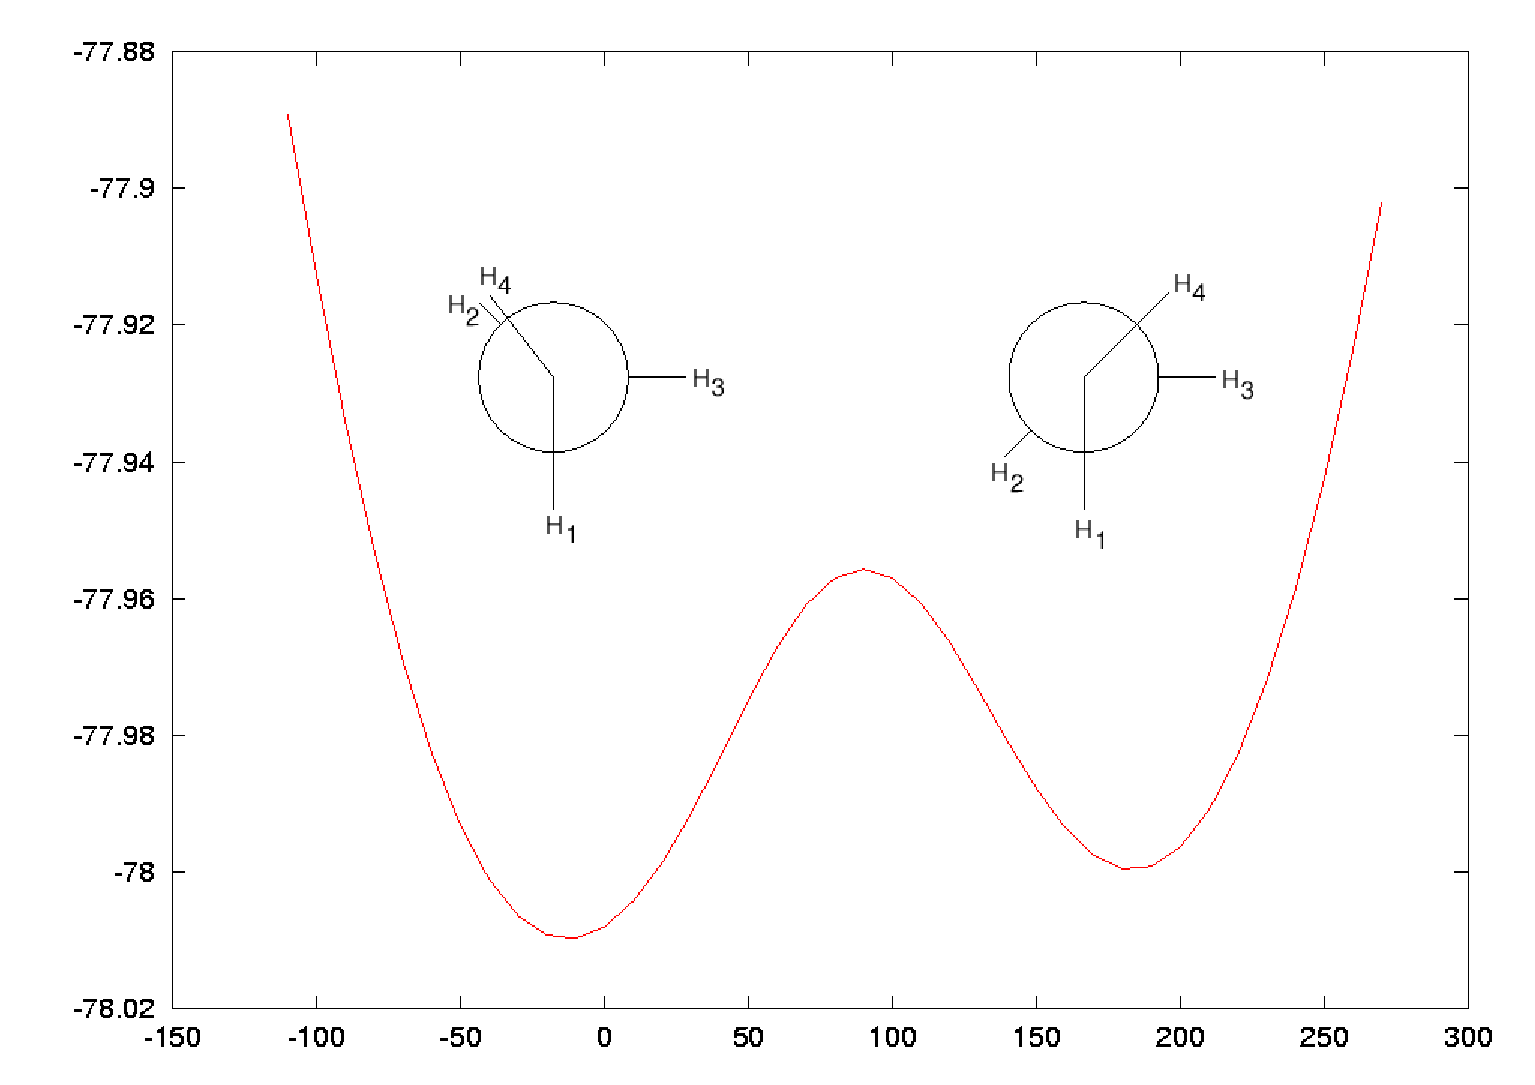
\includegraphics[angle=0,width=10cm,keepaspectratio]{immagini/etene/c090.eps}
\caption{\small Etilene - curva di potenziale rispetto all'angolo diedro
H$_2$-C-C-H$_4$. L'angolo diedro H$_1$-C-C-H$_3$ \`e fissato a 90$^{\circ}$}
\label{fig:etene_c090}
\end{center}
\end{figure}

Entrambi i minimi descrivono una possibile organizzazione spaziale a minima
energia della molecola in queste condizioni: la differenza, come \`e 
\begin{wrapfigure}{l}{6cm}
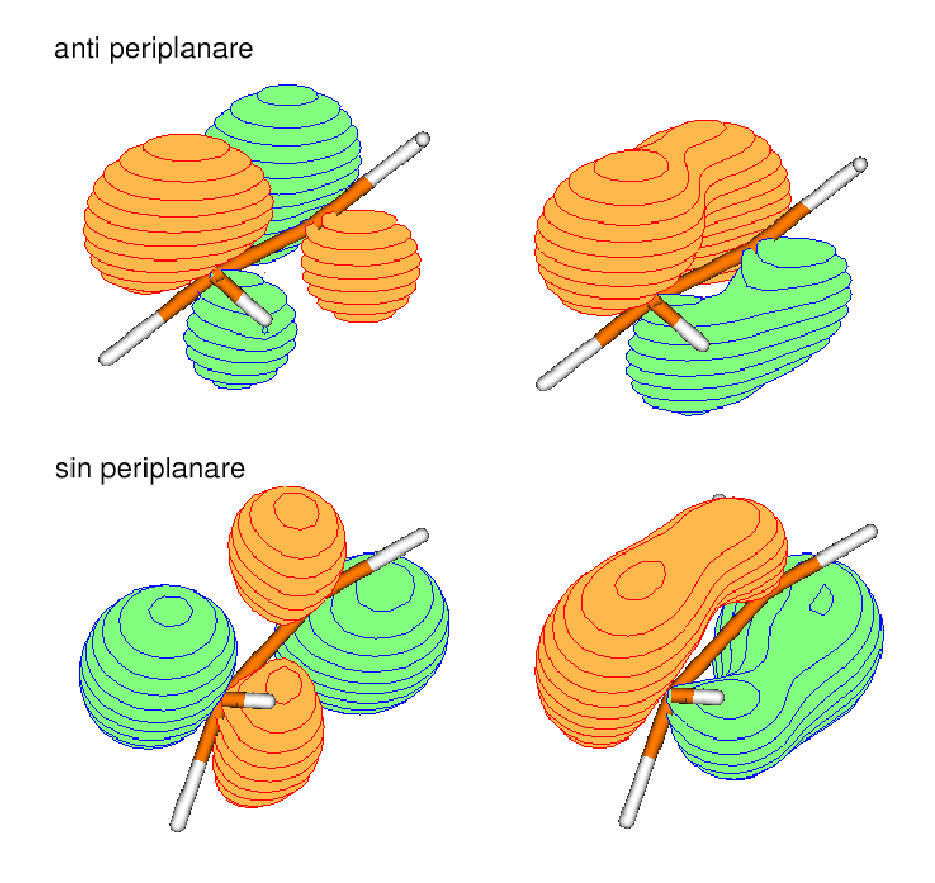
\includegraphics[angle=0,width=55mm,keepaspectratio]{immagini/etene/orbitali_c090.eps}
\caption{\small Etilene - orbitali dello spazio attivo (diedro H$_1$-C-C-H$_3$ a 90$^{\circ}$)}
\label{fig:etene_orbitali_c090}
\end{wrapfigure}
possibile notare dalla figura \ref{fig:etene_c090}, deriva dal diverso
posizionamento degli idrogeni H$_2$ e H$_4$, che assecondano i vincoli e la
necessit\`a di piramidalizzazione disponendosi in due diverse configurazioni
coplanari, una sin-periplanare, l'altra anti-periplanare. Il minimo
sin-periplanare possiede energia minore, anche a livello puramente nucleare,
sebbene presenti due atomi di idrogeno in posizione eclissata.
Gli orbitali attivi in queste due condizioni sono rappresentati in
figura \ref{fig:etene_orbitali_c090}.
La barriera di potenziale necessaria ad interconvertire, lungo questo grado
di libert\`a, la forma sin in forma anti \`e approssimativamente 1.45 eV, e passa per un
intermedio planare in cui gli orbitali $p$ degli atomi di carbonio sono
ortogonali.
L'utilizzo dell'etilene come esempio dimostrativo della superficie non
consente la distinzione tra isomero cis ed isomero trans, distinzione
che sar\`a apprezzabile nell'esatriene.


\subsection{Esatriene}

La molecola di esatriene \`e stata presa in esame sugli stessi parametri
dell'etilene, considerando la rotazione attorno al doppio legame centrale.

\begin{figure}[ht]
\begin{center}
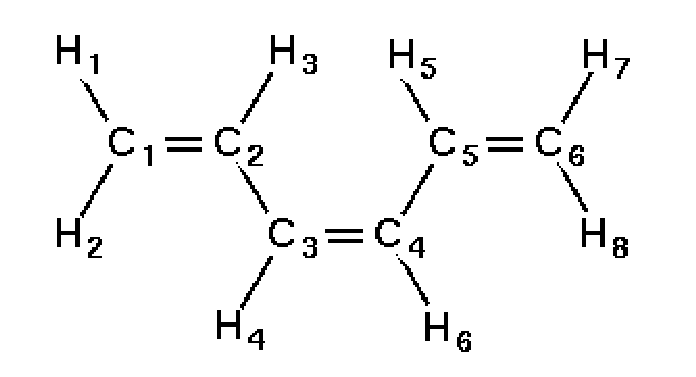
\includegraphics[angle=0,width=6cm,keepaspectratio]{immagini/esatriene/esatriene_cis.eps}
\end{center}
\end{figure}

Si \`e infatti valutata la superficie di potenziale associata ai due gradi di libert\`a
definiti dagli angoli diedri \mbox{C$_2$-C$_3$-C$_4$-C$_5$} e \mbox{H$_4$-C$_3$-C$_4$-H$_6$}.
La base usata per questa trattazione \`e la {6-31G*}. Lo spazio CAS \`e stato
definito in modo tale da includere 6 orbitali $\pi$ ed i corrispondenti
6 elettroni.
\begin{figure}[ht]
\begin{center}
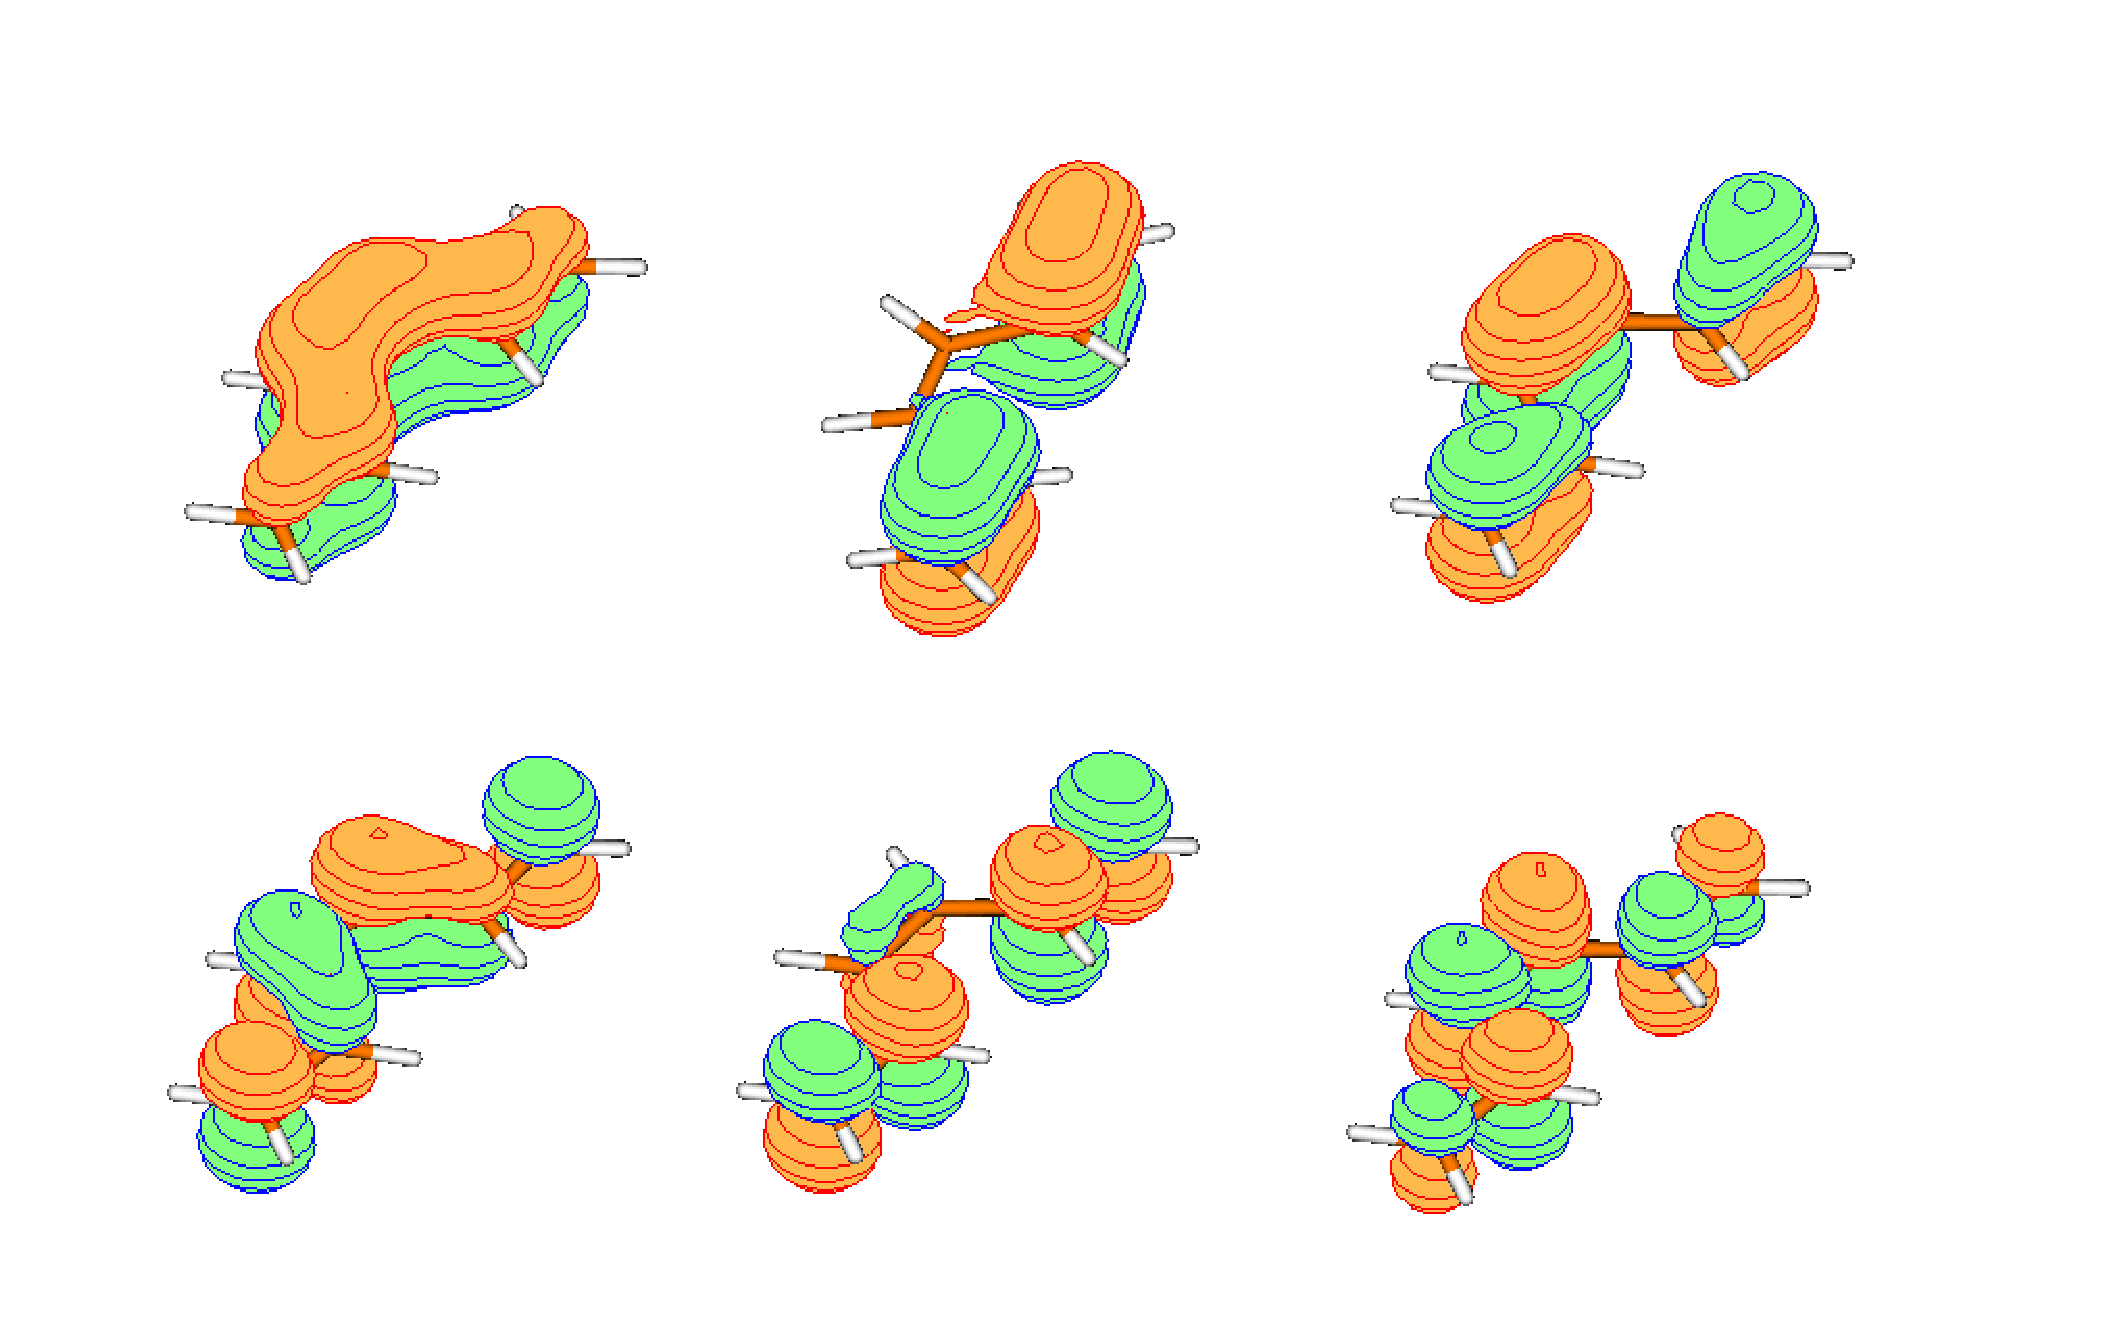
\includegraphics[angle=0,width=10cm,keepaspectratio]{immagini/esatriene/orbitali.eps}
\caption{\small Esatriene cis - orbitali nello spazio CAS 6/6}
\label{fig:esatriene_orbitali}
\end{center}
\end{figure}

\clearpage

La geometria dell'esatriene cis all'equilibrio \`e definita in tabella
\ref{tab:esatriene_geometrie}.
\begin{center}
\begin{threeparttable}
\caption{\small Esatriene cis - geometria stato fondamentale}
\label{tab:esatriene_geometrie}
\small
\begin{tabular}{|ccc|c|}
\hline
							& CASSCF	& Exp.\tnote{1} \\ 
\hline
$r$(C$_1$=C$_2$)			& 1.3456	& 1.336				\\
$r$(C$_2$-C$_3$)			& 1.4634	& 1.462				\\
$r$(C$_3$=C$_4$)			& 1.3537	& 1.362				\\
$r$(C$_1$-H$_1$)			& 1.0745	& 1.090				\\
$r$(C$_1$-H$_2$)			& 1.0763	& 1.090				\\
$r$(C$_2$-H$_3$)			& 1.0757	& 1.090				\\
$r$(C$_3$-H$_4$)			& 1.0775	& 1.090				\\
$\angle$(C$_1$C$_2$C$_3$)	& 123.293	& 122.1			 \\
$\angle$(C$_2$C$_3$C$_4$)	& 127.097	& 125.9		 \\
$\angle$(C$_2$C$_1$H$_1$)	& 121.546	& 124.0		 \\
$\angle$(C$_2$C$_1$H$_2$)	& 121.712	& 124.0		 \\
$\angle$(C$_4$C$_3$H$_4$)	& 117.476	& 118.0		 \\
$\angle$(C$_3$C$_2$H$_3$)	& 118.140	& 121.0		 \\
\hline
\end{tabular}
\begin{tablenotes}
\small
 \item[1] Cfr. \cite{jcp-114-4-2001-1631}
\end{tablenotes}
\end{threeparttable}
\end{center}

A tale geometria, ovviamente, gli angoli diedri \mbox{C$_2$-C$_3$-C$_4$-C$_5$} e
\mbox{H$_4$-C$_3$-C$_4$-H$_6$} sono entrambi pari a 0.

Successivamente si \`e proceduto ad effettuare la rotazione attorno al
doppio legame, facendo variare \mbox{C$_2$-C$_3$-C$_4$-C$_5$}. Per ragioni
strettamente numeriche la procedura seguita \`e stata differente da quella
ideale: dal punto di vista pratico si \`e partiti da una geometria gi\`a
ruotata, con diedro \mbox{C$_2$-C$_3$-C$_4$-C$_5$} pari a 90$^{\circ}$ e
diedro \mbox{H$_4$-C$_3$-C$_4$-H$_6$} pari a 0$^{\circ}$, e successivamente
si \`e effettuato un calcolo Restricted Open Shell. Questa procedura si \`e
resa necessaria per creare un buon set di orbitali da utilizzare nelle
successive ottimizzazioni. Utilizzando questo guess orbitalico si \`e quindi
effettuato il calcolo CASSCF alla medesima geometria, e si \`e fatto uso
degli orbitali ottenuti come guess per i successivi valori dell'angolo diedro
\mbox{H$_4$-C$_3$-C$_4$-H$_6$}.  La curva ottenuta \`e rappresentata in
figura \ref{fig:esatriene_c090}.

\begin{figure}[htb]
\caption{\small Esatriene - curva di potenziale rispetto al diedro
\mbox{H$_4$-C$_3$-C$_4$-H$_6$}, con diedro \mbox{C$_2$-C$_3$-C$_4$-C$_5$}
pari a 90$^{\circ}$}
\label{fig:esatriene_c090}
\begin{center}
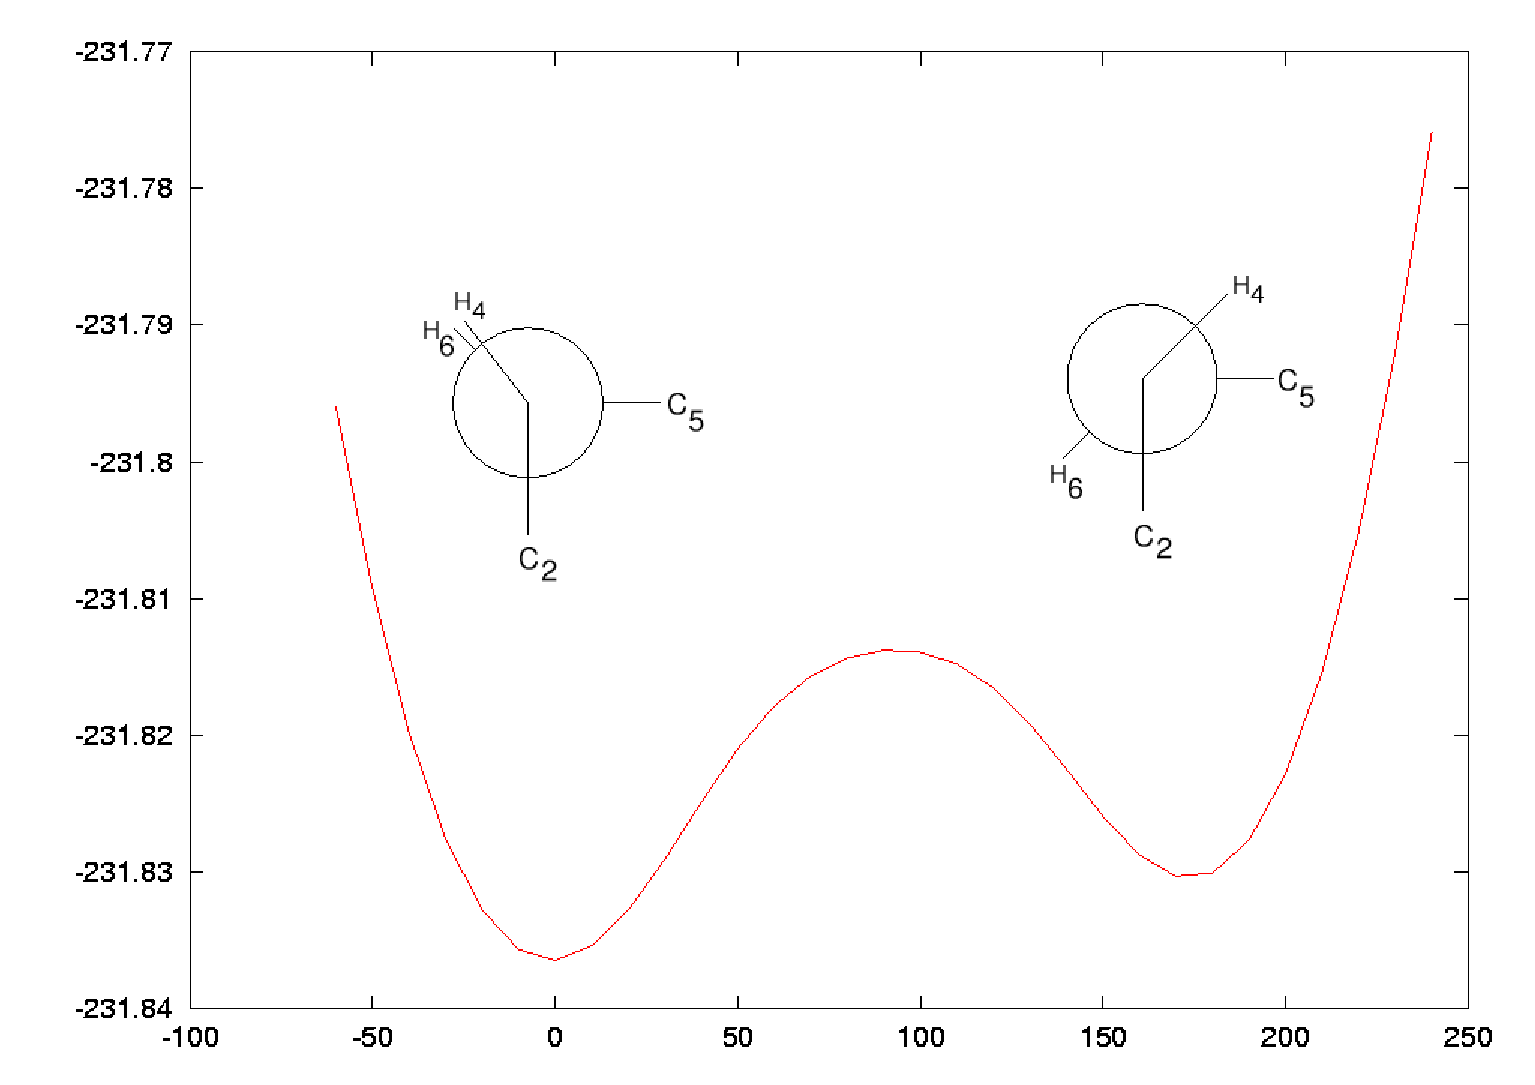
\includegraphics[width=10cm,keepaspectratio]{immagini/esatriene/c090.eps}
\end{center}
\end{figure}


Come \`e possibile notare, sono presenti due minimi, esattamente come nel
caso dell'etilene. Ciascun minimo rappresenta una possibile struttura di
equilibrio relativamente alla posizione degli idrogeni, una
approssimativamente sin-periplanare, l'altra approssimativamente
anti-periplanare. A differenza dell'etilene, tuttavia, \`e da notare che la
barriera di interconversione dalla sin alla anti \`e pi\`u bassa
(0.618 eV contro 1.45 eV per l'etilene). Questo \`e giustificabile
probabilmente in virt\`u della stabilizzazione dei due frammenti creati in
seguito alla rottura del doppio legame centrale. La formazione di due
frammenti vinilici contribuisce a ridurre l'energia della forma definita
dall'angolo diedro \mbox{H$_4$-C$_3$-C$_4$-H$_6$} a 90$^{\circ}$, in quanto tale forma
vede i frammenti privi di piramidalizzazione. Nel caso dell'etilene, si
ottenevano due orbitali $p$ completamente ortogonali che non potevano in
alcun modo interagire. Nel caso dell'esatriene e di tutti gli omologhi
superiori, ciascuno dei due orbitali \`e stabilizzato, e l'energia della
barriera risulta conseguentemente minore.

In queste condizioni, gli orbitali assumono combinazioni opportune: data la
simmetria C$_2$ della configurazione, si avranno combinazioni di simmetria
A o B sui gruppi di ciascun frammento.

Dal momento che ogni frammento pu\`o essere considerato un gruppo vinilico,
gli orbitali molecolari dello spazio attivo in questa situazione saranno 
definiti come in figura \ref{fig:esatriene_orbitali_c90_h90}
\pagebreak

\begin{figure}[htb]
\caption{\small Esatriene - spazio CAS per la configurazione con 
\mbox{H$_4$-C$_3$-C$_4$-H$_6$}=90$^{\circ}$ e
\mbox{C$_2$-C$_3$-C$_4$-C$_5$}=90$^{\circ}$ }
\label{fig:esatriene_orbitali_c90_h90}
\begin{center}
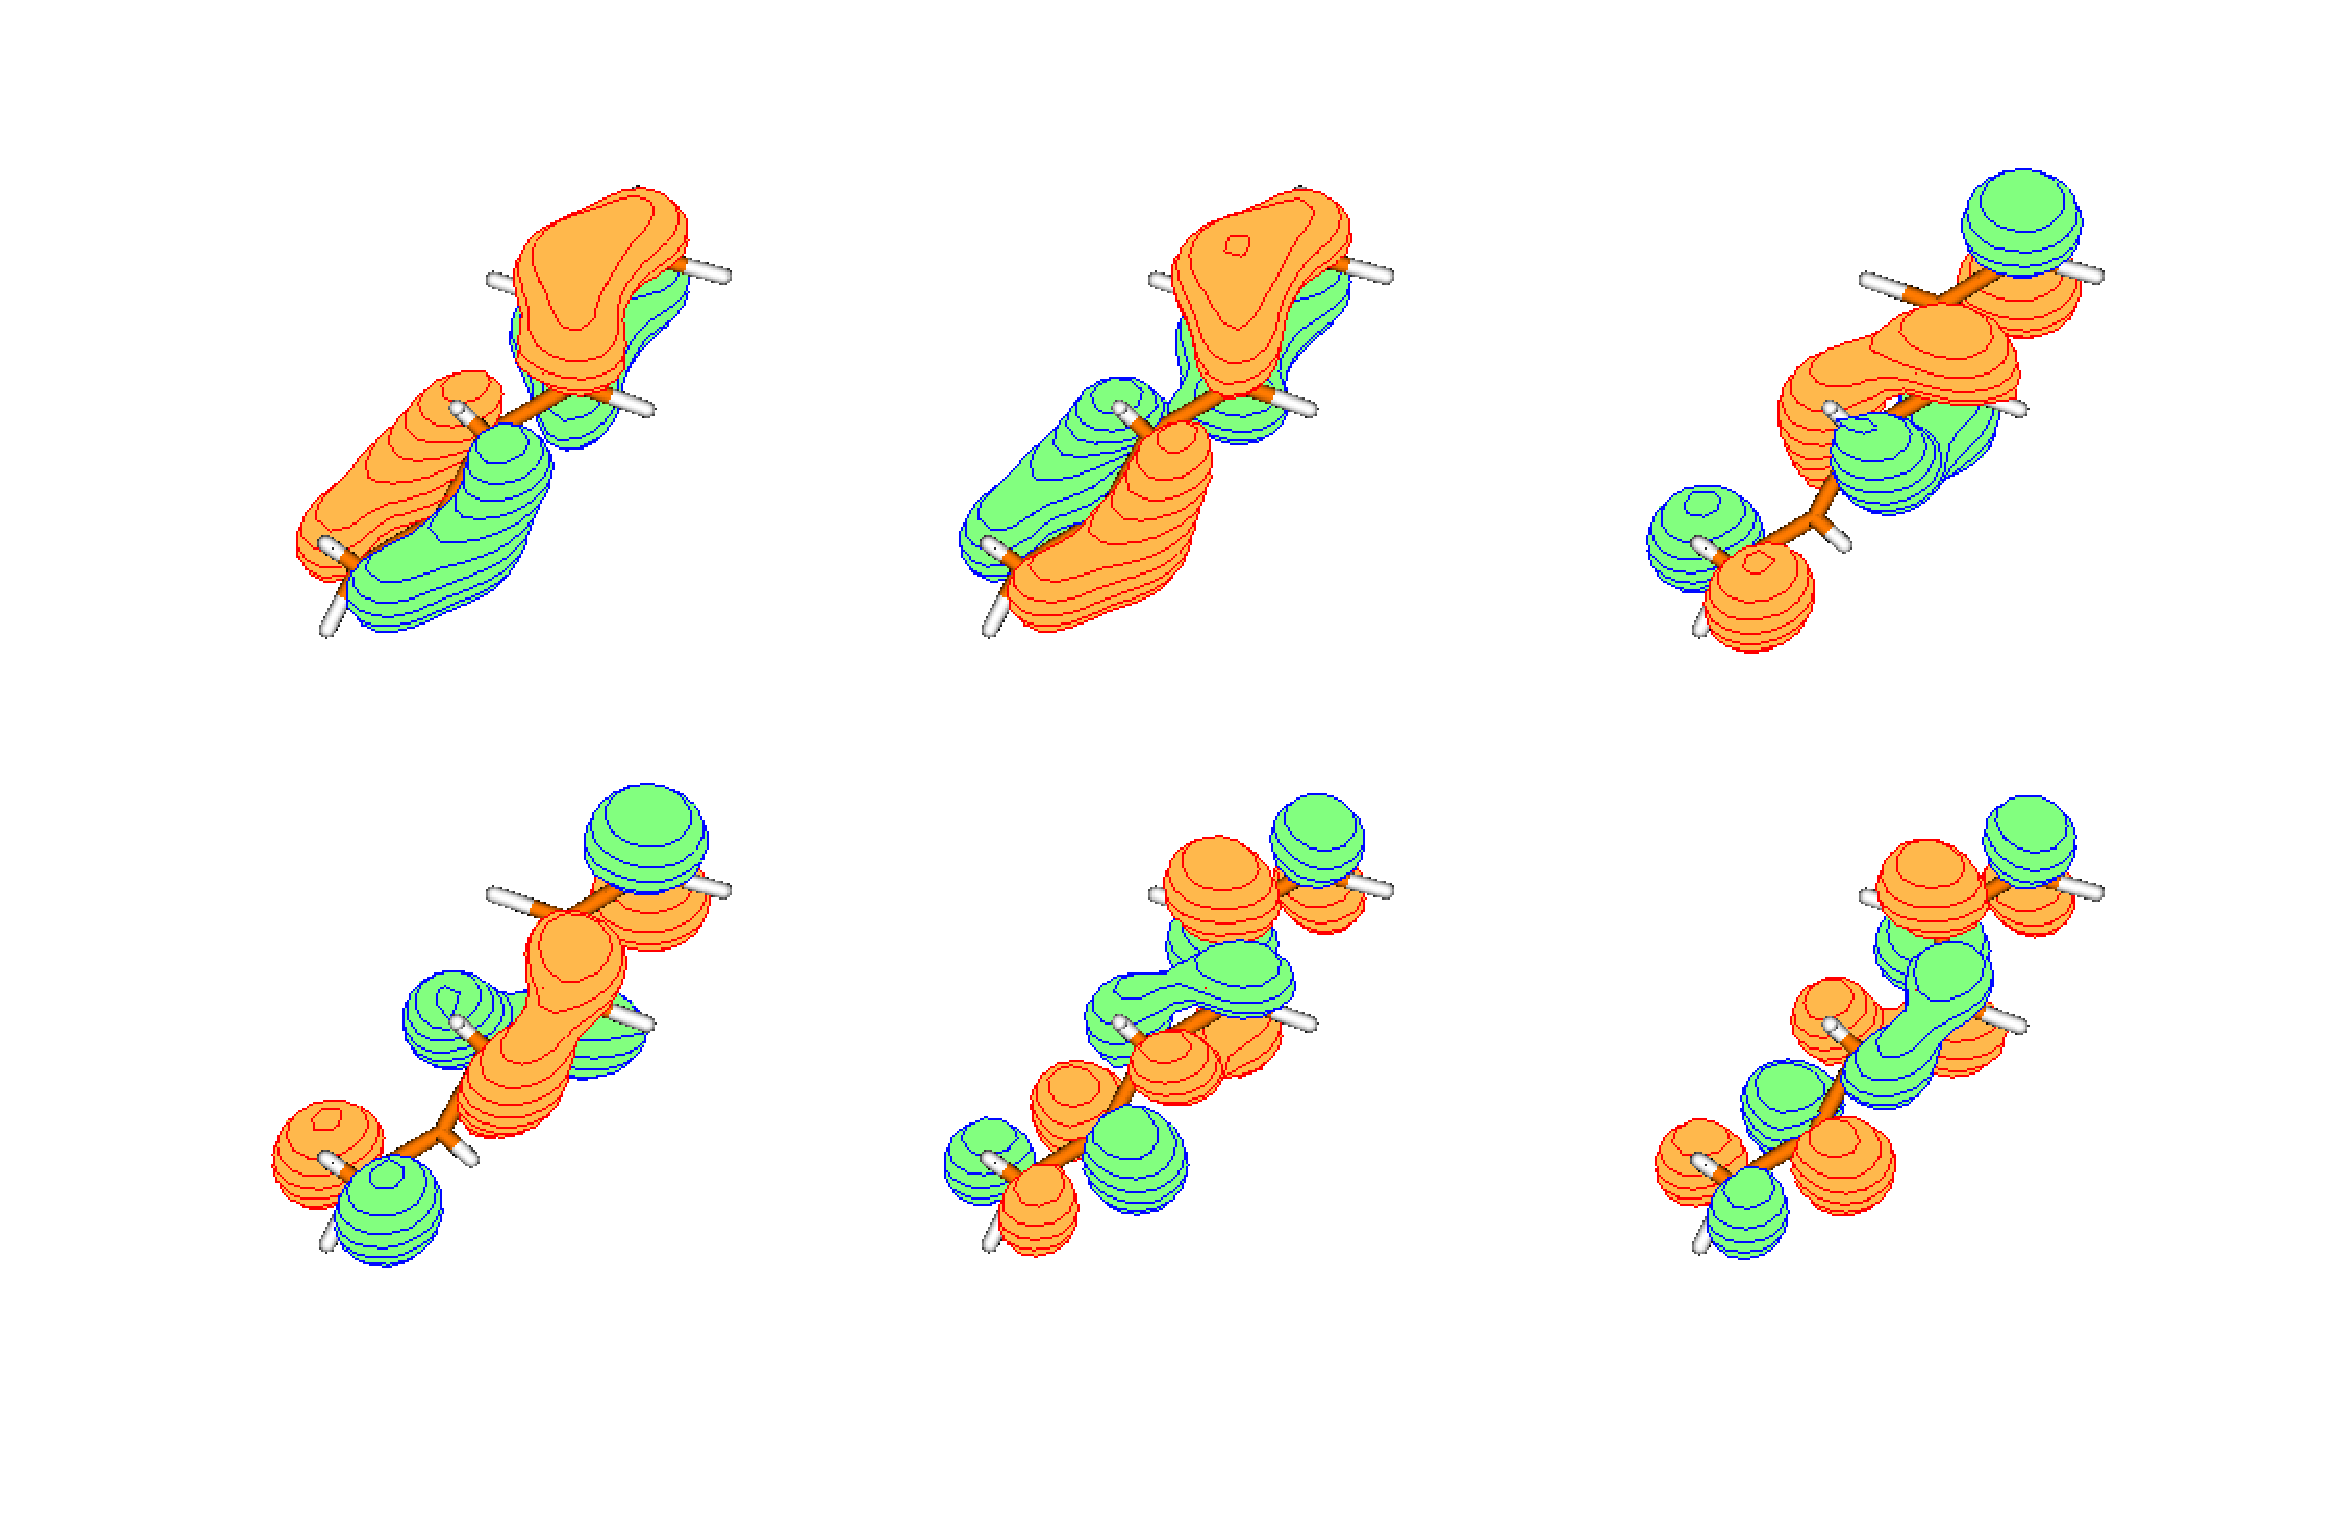
\includegraphics[width=12cm,keepaspectratio]{immagini/esatriene/orbitali_c90_h90.eps}
\end{center}
\end{figure}

Una volta ottenuto un set di orbitali per ogni posizione degli atomi di
idrogeno, si sono utilizzati come guess per ottenere le curve con angoli
diedri \mbox{C$_2$-C$_3$-C$_4$-C$_5$} inferiori e superiori di 90$^{\circ}$.

\begin{wrapfigure}{l}{8cm}
\includegraphics[angle=270,width=75mm,keepaspectratio]{immagini/esatriene/inviluppo.eps}
\caption{\small Esatriene - sezioni della superficie a vari angoli diedri C-C-C-C }
\label{fig:esatriene_inviluppo}
\end{wrapfigure}

Alcuni leggeri interventi si sono resi necessari nel caso che non si
ottenesse convergenza, tipicamente utilizzando il punto precedente o
successivo della curva. Alla fine si \`e ottenuta una superficie di
potenziale analoga a quella ottenuta per l'etilene ma, come gi\`a considerato
precedentemente, con una barriera a pi\`u bassa energia. 

\clearpage
\pagebreak

La superficie ottenuta si presta ad alcune considerazioni: \`e evidente che una
eventuale interconversione lungo questi gradi di libert\`a \`e difficilmente
realizzabile, sia perch\'e non vi \`e alcuna garanzia che questi gradi di
libert\`a siano gli unici in gioco nella interconversione, sia perch\'e questo
percorso prevede un forte spostamento di masse.

\begin{figure}[ht]
\begin{center}
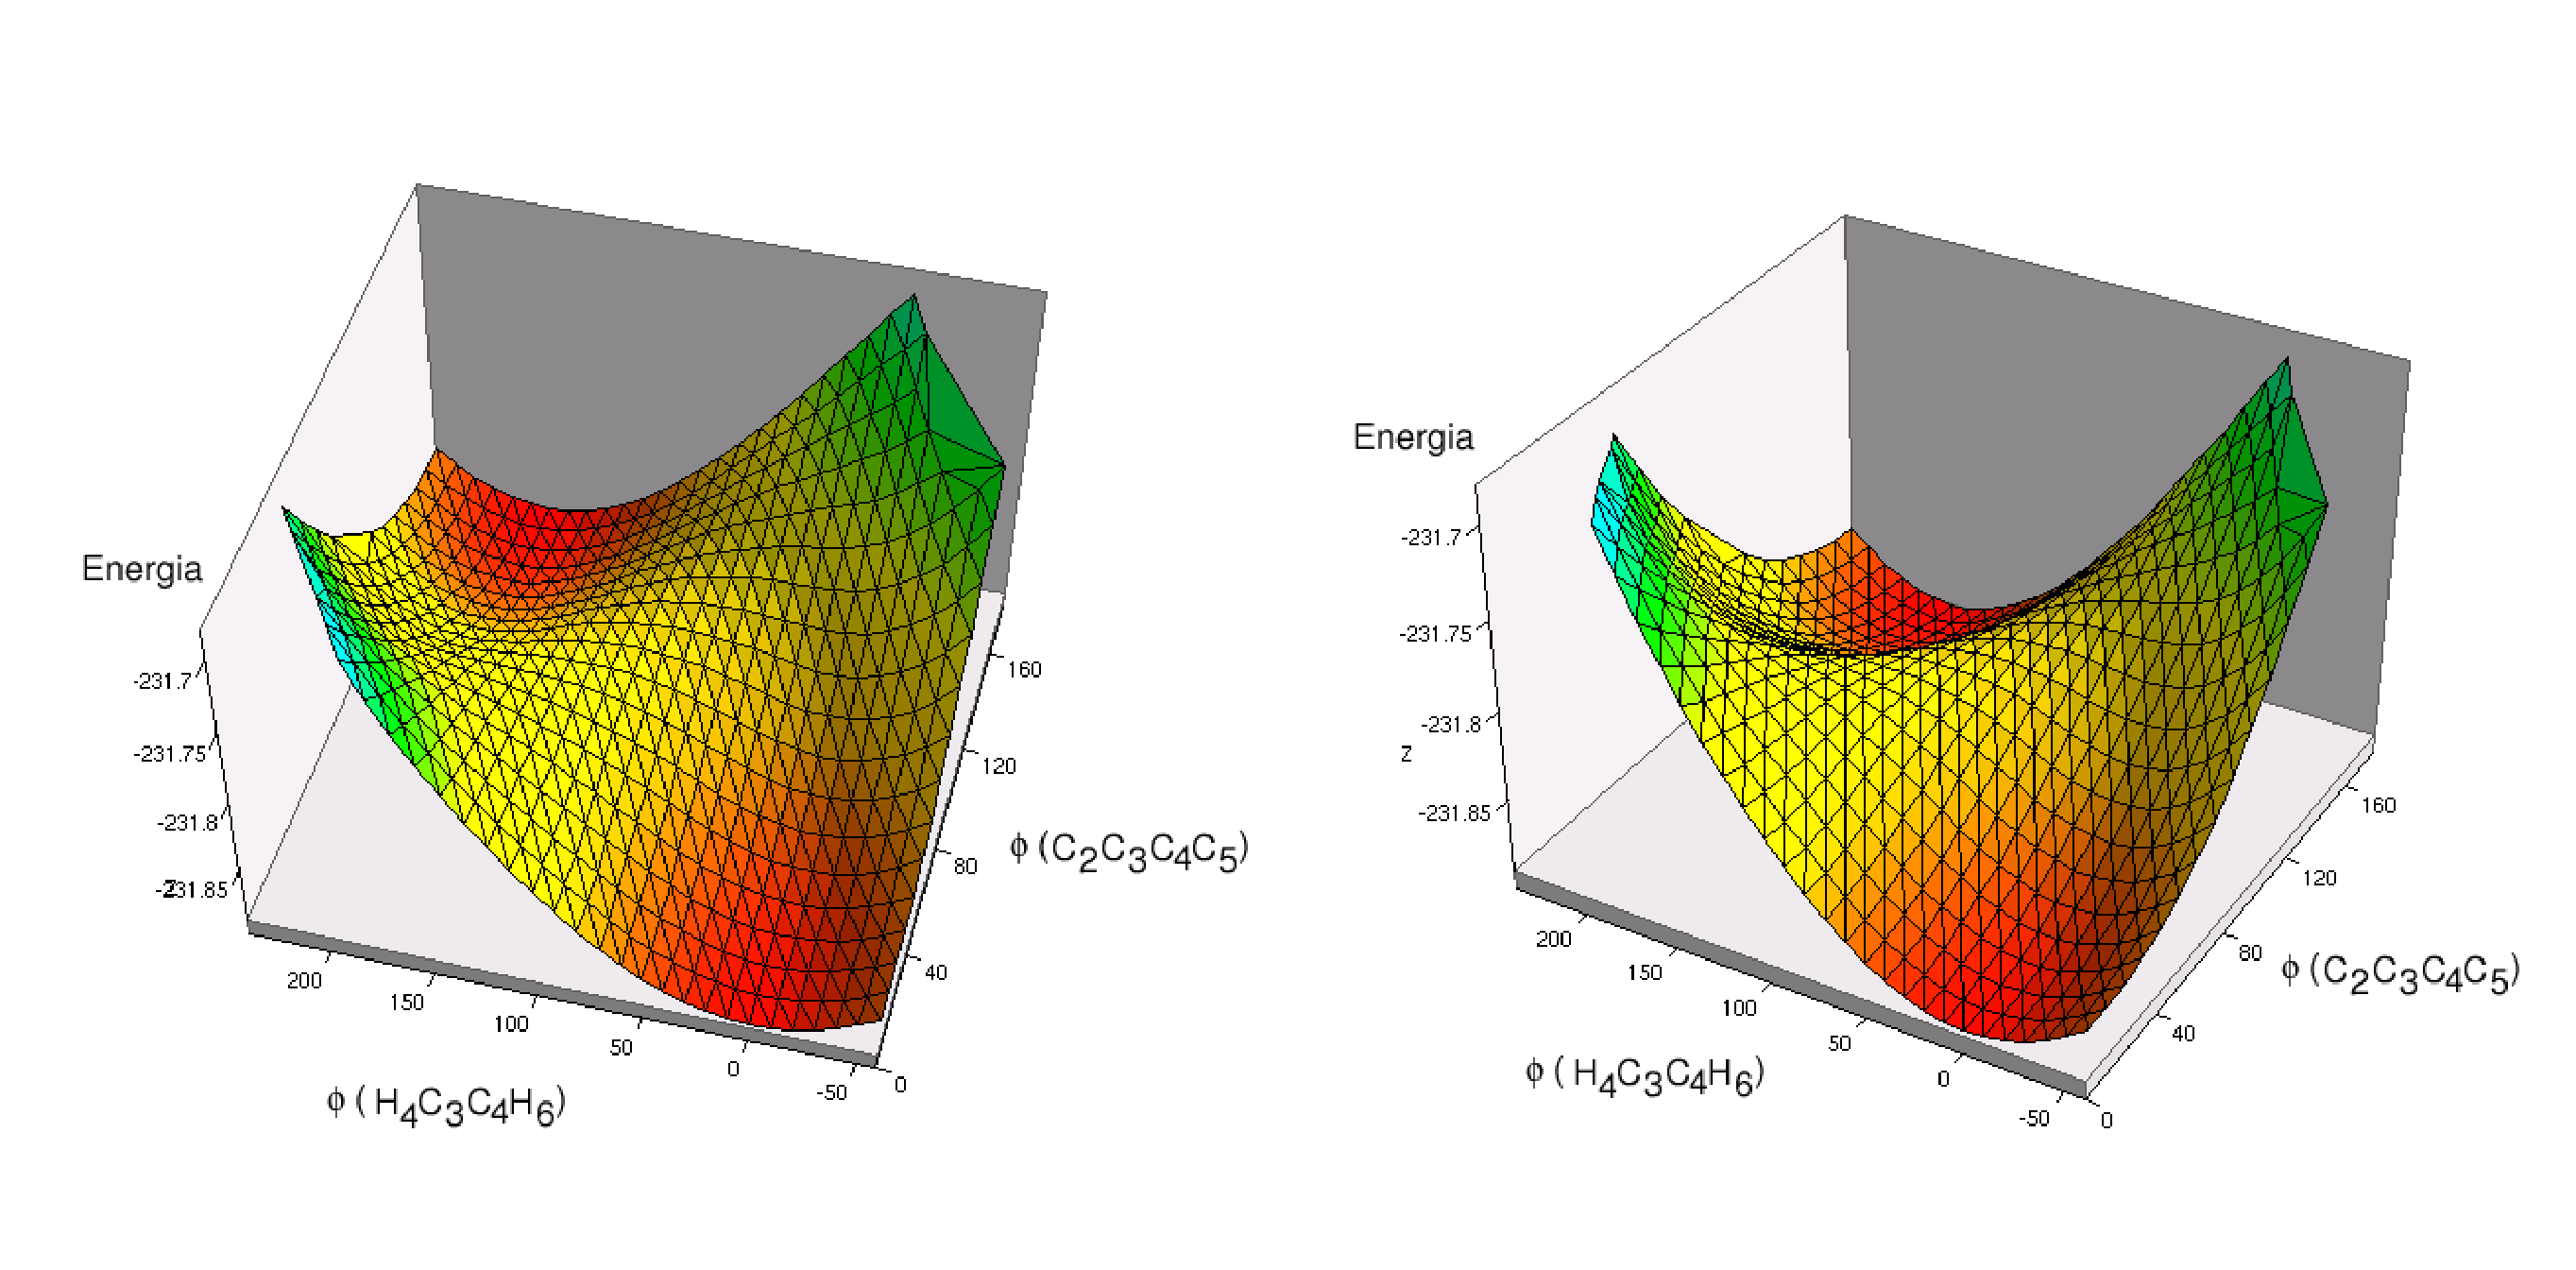
\includegraphics[angle=0,width=12cm,keepaspectratio]{immagini/esatriene/3d.eps}
\caption{\small Esatriene - superfici di potenziale}
\label{fig:esatriene_3d}
\end{center}
\end{figure}

Come conseguenza, difficilmente si tratta di una via di reale minimo energetico.
Nondimeno, una interconversione cis-trans che interessi esclusivamente lo stato
fondamentale deve necessariamente avvenire per via termica. Essendo i
polieni sistemi modello per molecole quali carotenoidi e acido retinoico,
precursori biologici di sistemi ad alta coniugazione responsabili di alcune
modalit\`a di pigmentazione e quali recettori luminosi, sar\`a centrale
nella loro interconversione il coinvolgimento di stati eccitati.
Tuttavia, \`e possibile evidenziare alcune caratteristiche interessanti:
\begin{itemize}
\item la forma sin periplanare correla, dal punto di vista strutturale, con
la forma cis del poliene. Al contrario la forma trans periplanare darebbe
origine ad un poliene i cui idrogeni centrali sono perpendicolari, e su
facce opposte, al piano molecolare, conformazione sicuramente non stabile,
come mostrato dalla ripidit\`a della curva a $\phi($C-C-C-C$) = 0^{\circ}$ e
$\phi($C-C-C-C$) = 180$.
\item analogamente, la forma trans-periplanare correla strutturalmente con
la forma trans del poliene. La forma cis-periplanare avrebbe sarebbe
analogamente non stabile, data la posizione degli idrogeni, ortogonali al
piano della molecola.
\item L'interconversione dalla forma cis ($\phi($C-C-C-C$) = 0^{\circ}$) alla forma
trans ($\phi($C-C-C-C$) = 180^{\circ}$) del poliene lungo i gradi di libert\`a definiti
impone un salto di una barriera energetica la cui altezza diminuisce via via
che l'angolo diedro $\phi($C-C-C-C$)$ aumenta. Questa barriera tende ad una
spalla che forza la risoluzione della specie verso la forma quasi
periplanare pi\`u stabile, in questo caso la trans. Analogo comportamento si
ottiene nell'interconversione dalla specie trans alla specie cis.
\end{itemize}

In virt\`u di quest'ultimo punto, il percorso di interconversione cis-trans
\`e differente dal percorso trans-cis. La molecola tende a seguire il minimo
locale della struttura che correla al meglio con lo stato di partenza, fino
a quando tale struttura non fornisce pi\`u uno stato di minimo energetico.
Quando ci\`o avviene, la struttura evolve verso lo stato di minimo energetico
modificando opportunamente la posizione degli idrogeni.

La figura \ref{fig:esatriene_mep_1} mostra i due differenti percorsi di
interconversione. Con la griglia di punti attuata per questa descrizione
(ogni 10 gradi del diedro tra i carboni)  \`e difficile localizzare dove
avvenga il rilassamento alla struttura geometricamente pi\`u stabile. Una
ulteriore difficolt\`a deriva dalla lentissima convergenza del calcolo di
ottimizzazione geometrica nelle vicinanze della spalla, punto nel quale il
gradiente \`e quasi nullo e, di conseguenza, l'eventuale riarrangiamento
verso il minimo assoluto procede molto lentamente.
La figura \ref{fig:esatriene_punti_minimo} fa riferimento alla posizione di
tali punti sul piano dei diedri.
\begin{figure}[ht]
\begin{center}
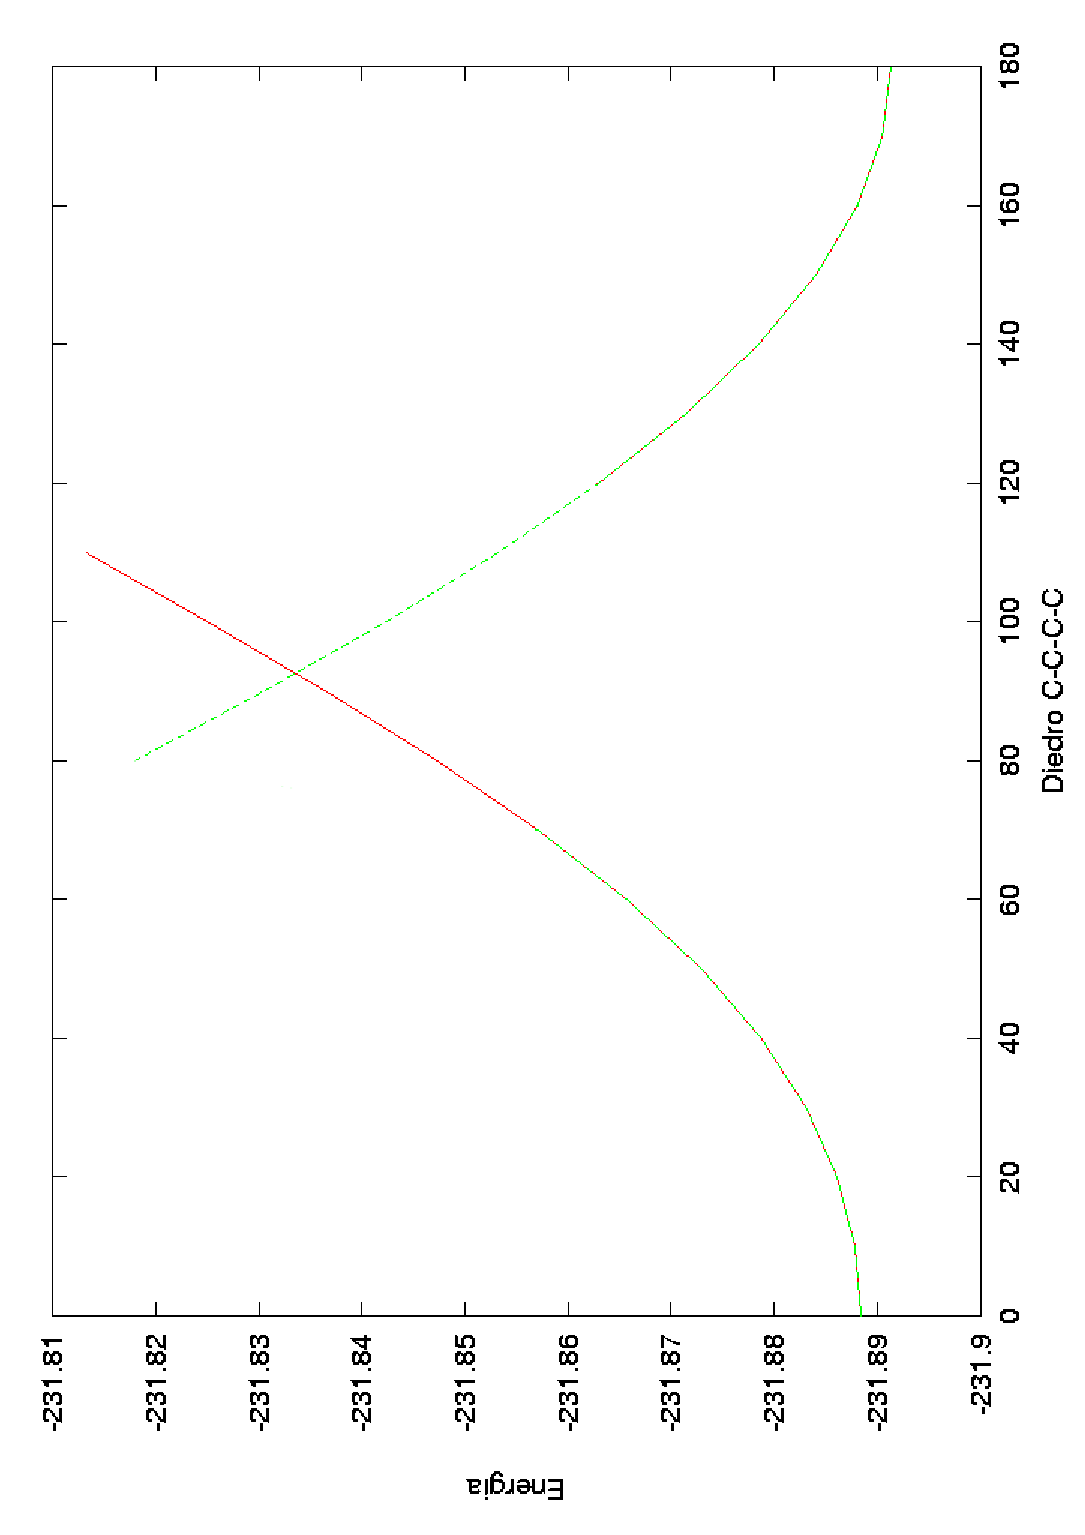
\includegraphics[angle=270,width=10cm,keepaspectratio]{immagini/esatriene/mep_1.eps}
\caption{\small Esatriene - percorso a minima energia lungo i gradi di
libert\`a definiti. Energie assolute}
\label{fig:esatriene_mep_1}
\end{center}
\end{figure}
\clearpage

\begin{figure}[ht]
\begin{center}
\includegraphics[angle=270,width=12cm,keepaspectratio]{immagini/esatriene/punti_minimo.eps}
\caption{\small Esatriene - percorso a minima energia lungo i gradi di
libert\`a definiti. Posizione sul piano definito dai diedri}
\label{fig:esatriene_punti_minimo}
\end{center}
\end{figure}

\`E quindi possibile approssimativamente definire tali punti di
interconversione in un intervallo compreso tra 70-80$^{\circ}$ per il mep
trans-cis e 110-120$^{\circ}$ per il mep cis-trans.

\subsubsection{Analisi perturbativa NEV-PT}

Successivamente allo studio approfondito a livello CASSCF, si \`e valutata
la variazione della struttura della superficie in seguito alla trattazione
perturbativa NEV-PT.

Sono state studiate le curve di potenziale rispetto al diedro H-C-C-H,
con angolo diedro C-C-C-C fissato a 0, 90 e 180$^{\circ}$. Tutte le
curve perturbative sono state traslate con opportuni valori al
fine di confrontarle dal punto di vista strutturale. Tali valori sono
di 0.710535 Hartree per le curve della trattazione strongly contracted e
0.710911 Hartree per le curve della partially contracted, valori che
rappresentano lo scarto tra le curve perturbative e la curva CASSCF nel 
punto con diedri C-C-C-C e H-C-C-H uguali a zero (ovvero la condizione di
equilibrio per l'isomero cis). 

L'analisi dell'andamento della perturbazione sulla curva a 0$^{\circ}$ ha
fornito il risultato in figura \ref{fig:esatriene_perturb_c0}.
Come si pu\`o notare, l'effetto perturbativo non introduce variazioni
nell'andamento della curva, ma si limita ad effettuare una traslazione
energetica dovuta al migliore contributo correlativo. In altri termini, il
contributo correlativo fornito dalla NEV-PT sulla funzione CASSCF \`e
uniforme per ogni punto della curva.

\begin{figure}[ht]
\begin{center}
\includegraphics[angle=270,width=12cm,keepaspectratio]{immagini/esatriene/perturb_c0.eps}
\caption{\small Esatriene - curva CASSCF (in rosso) con diedro C-C-C-C = 0$^{\circ}$, e curve perturbative
strongly (in verde) e partially (in blu), queste ultime traslate di 0.710535 e 0.710911 Hartree rispettivamente. Le
curve sono praticamente sovrapposte.}
\label{fig:esatriene_perturb_c0}
\end{center}
\end{figure}

Risultato molto simile si \`e ottenuto per la curva a 180$^{\circ}$, visibile
in figura \ref{fig:esatriene_perturb_c180}. In tale condizione \`e possibile
notare come il contributo perturbativo innalzi leggermente l'energia della
condizione pi\`u sfavorevole, ovvero quella per l'isomero trans con idrogeni
quasi ortogonali.

\begin{figure}[ht]
\begin{center}
\includegraphics[angle=270,width=12cm,keepaspectratio]{immagini/esatriene/perturb_c180.eps}
\caption{\small Esatriene - curva CASSCF (in rosso) con diedro C-C-C-C = 180$^{\circ}$, e curve perturbative
strongly (in verde) e partially (in blu), queste ultime traslate di 0.710535 e 0.710911 Hartree rispettivamente.}
\label{fig:esatriene_perturb_c180}
\end{center}
\end{figure}

Per quanto riguarda infine la curva con diedro C-C-C-C = 90$^{\circ}$,
incontriamo invece un certo cambiamento ad opera della trattazione
perturbativa: la barriera si innalza e si restringe, cos\`i come anche le due
buche di potenziale caratterizzanti i due stati coplanari per gli idrogeni. 

\begin{figure}[ht]
\begin{center}
\includegraphics[angle=270,width=12cm,keepaspectratio]{immagini/esatriene/perturb_c90.eps}
\caption{\small Esatriene - curva CASSCF (in rosso) con diedro C-C-C-C = 90$^{\circ}$, e curve perturbative
strongly (in verde) e partially (in blu), queste ultime traslate di 0.710535 e 0.710911 Hartree rispettivamente.}
\label{fig:esatriene_perturb_c90}
\end{center}
\end{figure}

\clearpage
\pagebreak

Il programma \texttt{dypc2} fornisce, nell'output, dettagli sul contributo
(come norma della correzione al primo ordine alla funzione d'onda e come energia)
sia per la correzione parzialmente contratta che
per quella fortemente contratta. Nelle figure \ref{fig:esatriene_norme_sc},
\ref{fig:esatriene_norme_pc}, \ref{fig:esatriene_energie_sc} e
\ref{fig:esatriene_energie_pc} sono mostrati rispettivamente gli andamenti,
rispetto al diedro H-C-C-H, dei valori delle norme strongly e partially e
delle correzioni alle energie strongly e partially, con diedro C-C-C-C
fissato a 90$^{\circ}$.

\`E possibile notare come il maggiore contributo alla correzione perturbativa
venga portato principalmente da $V(0)$ e $V(0')$, denotando chiaramente come 
le doppie eccitazioni siano fondamentali per la descrizione della molecola. %(Cfr. \cite{jcp-114-4-2001-1631} e \cite{jcp-112-2-2000-613})

\pagebreak
\begin{figure}[ht]
\begin{center}
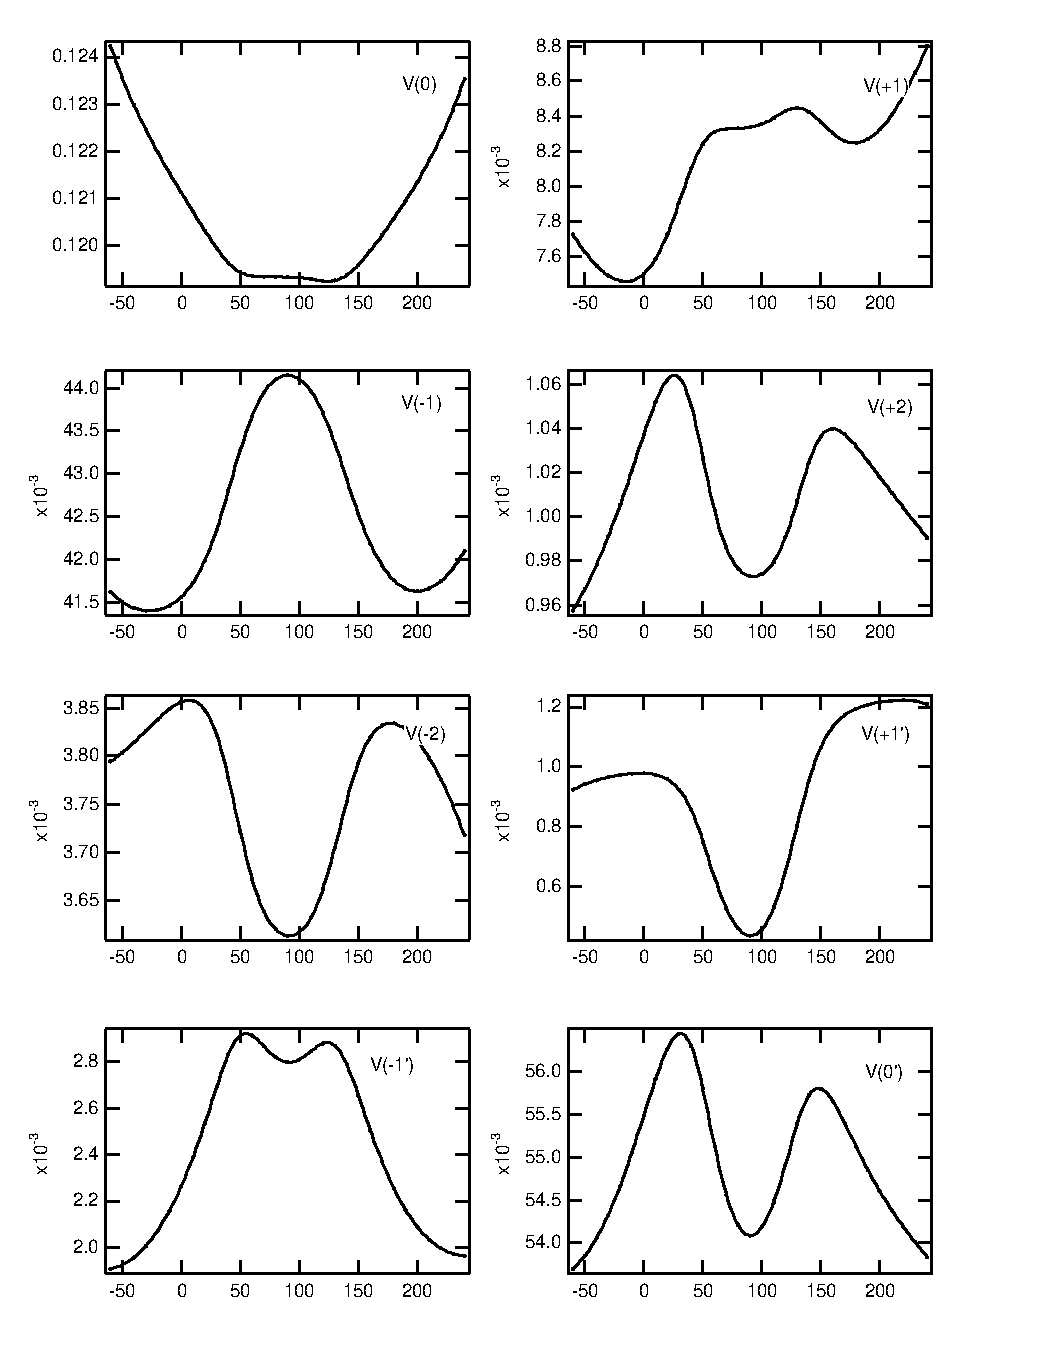
\includegraphics[angle=0,width=14cm,keepaspectratio]{immagini/esatriene/norme_sc.eps}
\caption{\small Esatriene - Norme per la correzione alla funzione d'onda.
Trattazione strongly contracted. }
\label{fig:esatriene_norme_sc}
\end{center}
\end{figure}
\pagebreak
\begin{figure}[ht]
\begin{center}
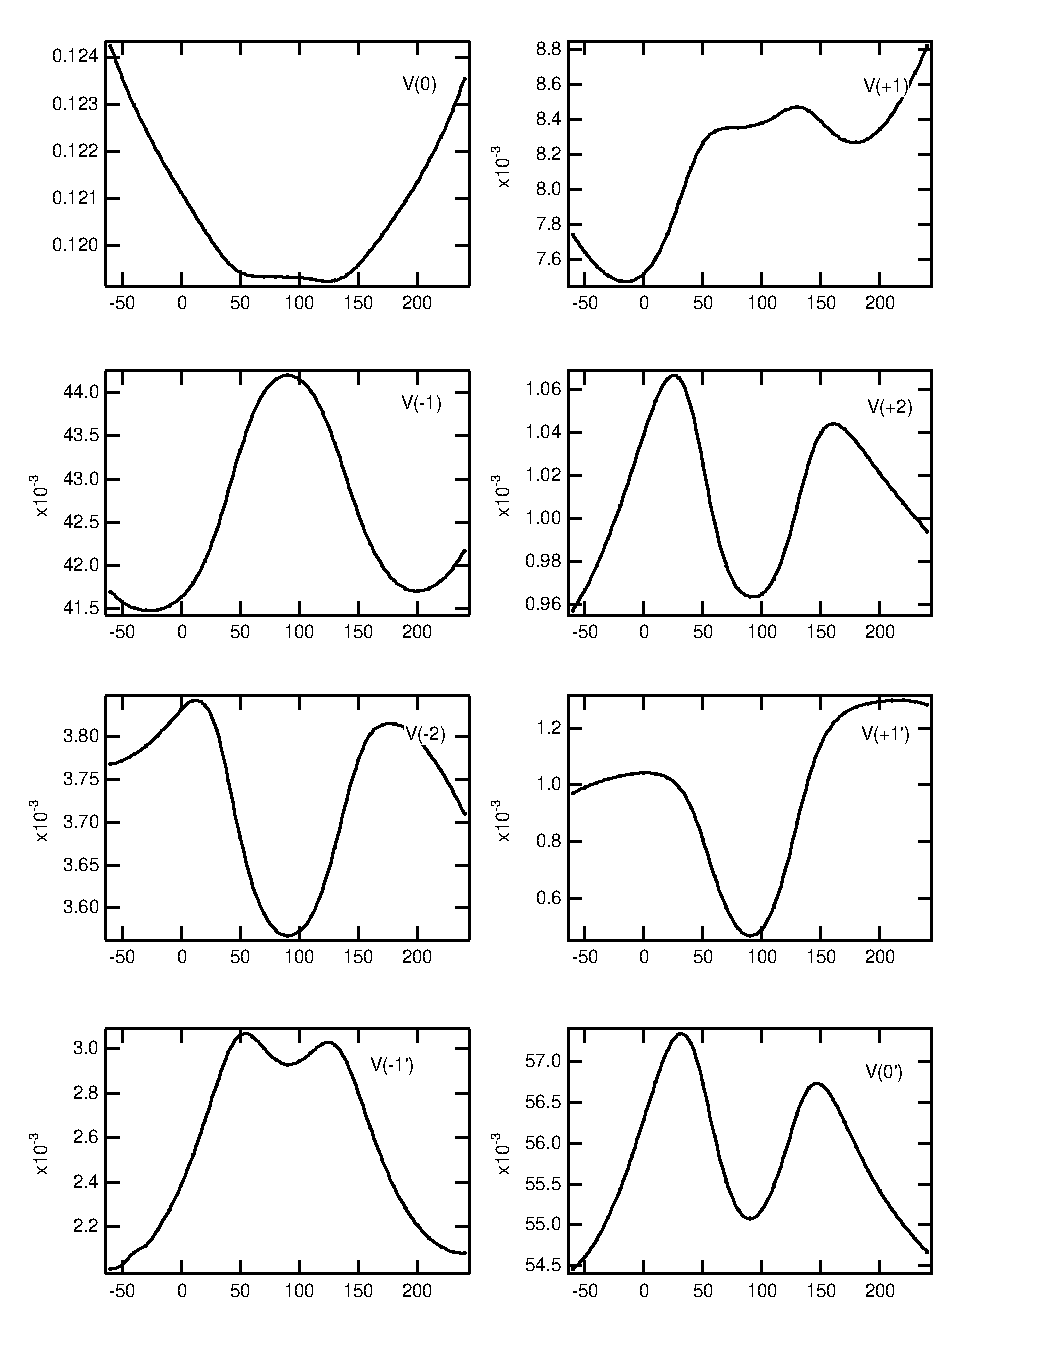
\includegraphics[angle=0,width=14cm,keepaspectratio]{immagini/esatriene/norme_pc.eps}
\caption{\small Esatriene - Norme per la correzione alla funzione d'onda.
Trattazione partially contracted. }
\label{fig:esatriene_norme_pc} 
\end{center}
\end{figure}
\pagebreak
\begin{figure}[ht]
\begin{center}
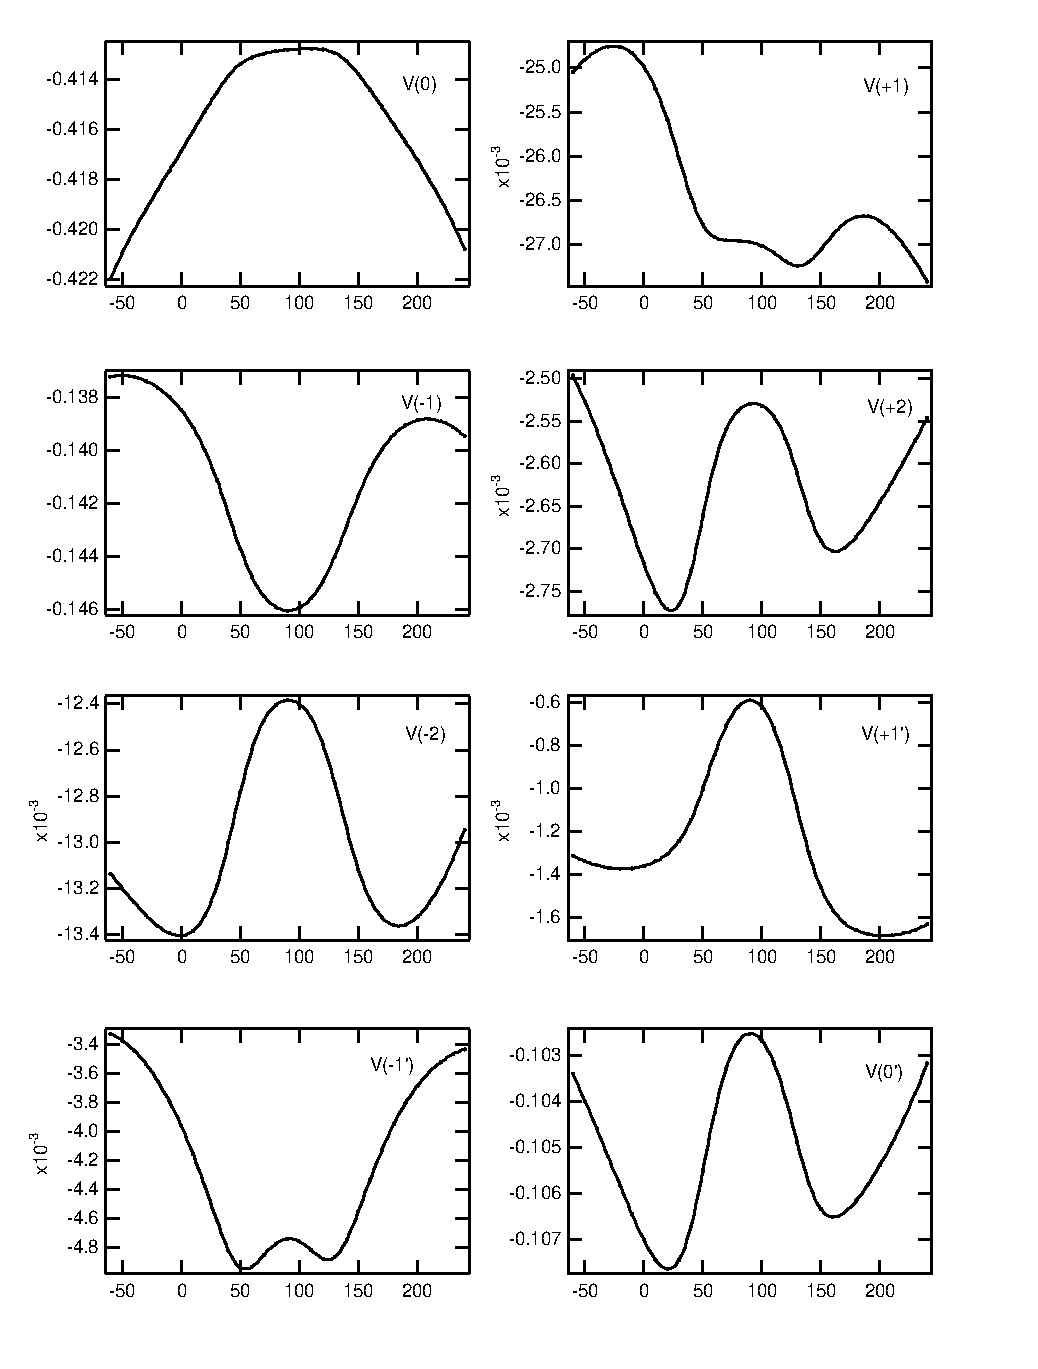
\includegraphics[angle=0,width=14cm,keepaspectratio]{immagini/esatriene/energie_sc.eps}
\caption{\small Esatriene - Contributi all'energia per l'applicazione
strongly contracted. Valori in Hartree. }
\label{fig:esatriene_energie_sc}
\end{center}
\end{figure}
\pagebreak
\begin{figure}[ht]
\begin{center}
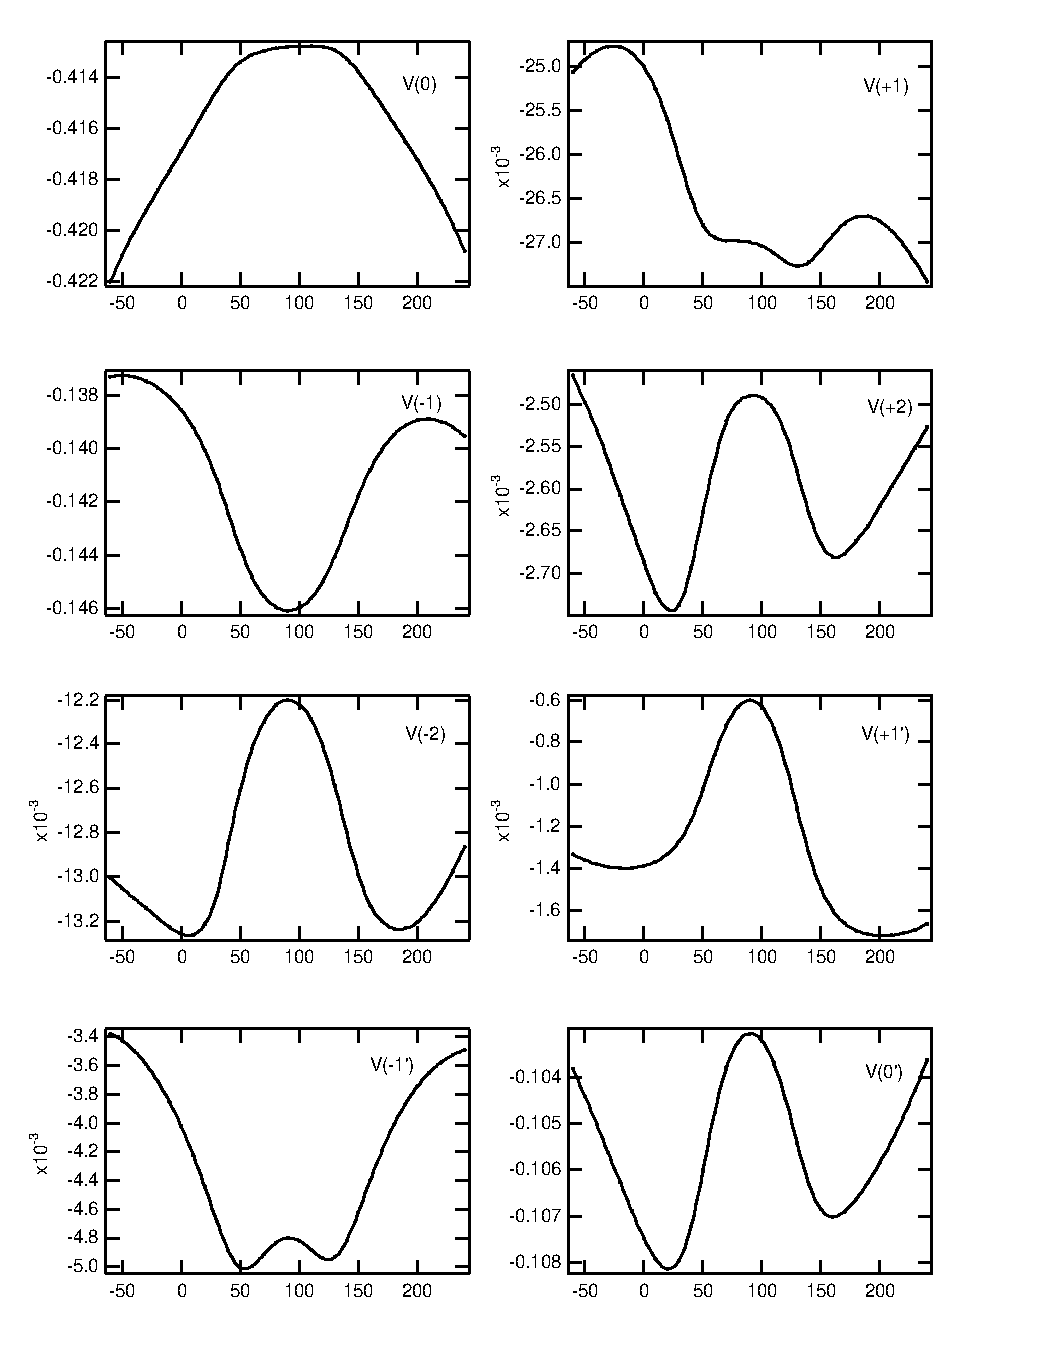
\includegraphics[angle=0,width=14cm,keepaspectratio]{immagini/esatriene/energie_pc.eps}
\caption{\small Esatriene - Contributi all'energia per l'applicazione
partially contracted. Valori in Hartree. }
\label{fig:esatriene_energie_pc}
\end{center}
\end{figure}
\pagebreak

\clearpage

\subsubsection{Energie di eccitazione verticale}

Sempre sulla molecola di esatriene si sono effettuati calcoli di valutazione
dell'energia di eccitazione verticale sia sull'isomero cis che sull'isomero
trans.

L'isomero cis, con simmetria $C_{2v}$, \`e stato ottimizzato con base 6-31G*
a livello CAS. Lo spazio attivo \`e costituito dai 6 elettroni
negli orbitali di natura $\pi$, orbitali appartenenti alle rappresentazioni
B$_1$ e A$_2$. La trattazione ha richiesto 92 configurazioni.
Al termine della procedura CASSCF, i numeri di occupazione per lo stato
fondamentale erano i seguenti
\begin{verbatim}
 Simmetria B1

   1.937856768   1.862253783   0.085298882

 Simmetria A2

   1.913147630   0.144502101   0.056940836
\end{verbatim}

Alla medesima geometria \`e stato condotto successivamente il calcolo per lo
stato eccitato 2A$_1$. I numeri di occupazione risultano essere
\begin{verbatim}
 Simmetria B1

   1.836468224   1.016224575   0.339483529

 Simmetria A2

   1.661825866   1.015253102   0.130744704
\end{verbatim}

\`E evidente la diversa distribuzione elettronica in questo stato eccitato.
A questo livello, l'energia di transizione risulta essere di 5.71 eV. Il
valore sperimentale \`e incerto, sebbene esistano alcuni riferimenti
(Cfr. \cite{jcp-114-4-2001-1631}) che forniscono un range da 4.57 a 5.04 eV.
Applicando la trattazione perturbativa, il risultato non cambia
notevolmente: l'approccio strongly contracted fornisce 5.69 eV, mentre il
partially contracted 5.67 eV. 

La medesima procedura \`e stata svolta per l'isomero trans, di simmetria
C$_{2h}$, relativamente allo stato eccitato 2$A_g$. Riferimenti esistenti
forniscono valori approssimativi, che spaziano in un range da
4.26 fino anche a 6.45 eV (vedere \cite{pccp-3-2001-2567}, \cite{jcp-112-2-2000-613},
\cite{jcp-92-1990-4622}). Il calcolo \`e stato condotto su base 6-31G* con
spazio CAS 6/6, ed il risultato ottenuto \`e 5.68 eV. A livello perturbativo,
il risultato resta sostanzialmente invariato: 5.68 eV su strongly contracted e
5.67 eV su partially.

Al fine di valutare meglio questa transizione, si \`e fatto uso di uno spazio
CAS espanso, ottenuto aggiungendo un orbitale virtuale per ogni simmetria.
In seguito a tale variazione, per descrivere il sistema sono ora necessarie
600 configurazioni per entrambi gli isomeri, contro le 92 dello spazio CAS
precedente.

La transizione per l'isomero cis fornisce, a livello CASSCF, 5.72 eV, e i
valori ricavati dalla trattazione perturbativa sono 5.74 e 5.72 eV, 
rispettivamente per strongly e partially.
L'isomero trans invece fornisce 5.69 eV, 5.73 e 5.70 rispettivamente per
CASSCF, strongly e partially.


